\documentclass[letterpaper,12pt,oneside,final]{book}
%%
%%  Gabarit bilingue de mémoire de maîtrise ou thèse de doctorat.
%%  Bilingual template for dissertations and theses @ Polytechnique Montreal.

%%  Normalement, il n'est pas nécessaire de modifier ce document
%%  sauf pour établir le langage (français ou anglais) et pour changer les noms des fichiers à inclure.
%%  Usually, this document needs to be modified only to set up the language (French or English) and to change the names of the files to include.
%%
%%  Version: 2022-06-7
%%
%% Accepte les caractères accentués dans le document (UTF-8).
%% Supports accented characters in the document (UTF-8).

% make it a little easier on the eyes
\usepackage{xcolor}
\pagecolor[rgb]{0,0,0} %black
\color[rgb]{0.5,0.5,0.5} %grey
% end revert color, comment before print

\makeatletter
\def\bstctlcite{\@ifnextchar[{\@bstctlcite}{\@bstctlcite[@auxout]}}
\def\@bstctlcite[#1]#2{\@bsphack
 \@for\@citeb:=#2\do{%
   \edef\@citeb{\expandafter\@firstofone\@citeb}%
   \if@filesw\immediate\write\csname #1\endcsname{\string\citation{\@citeb}}\fi}%
 \@esphack}
\makeatother

%% LA COMMANDE SUIVANTE ÉTABLIT LE LANGAGE DE LA THÈSE : ÉCRIRE french POUR UNE THÈSE EN FRANÇAIS
%% THE NEXT COMMAND DETERMINES THE LANGUAGE OF THE THESIS: WRITE english FOR A THESIS IN ENGLISH
\newcommand\Langue{french}            

\usepackage{ifthen}
\usepackage[utf8]{inputenc}
%%
%% Support pour l'anglais et le français (français par défaut).
%% Support for English and French (French by default).

%\usepackage[cyr]{aeguill}
\usepackage{lmodern}      % Police de caractères plus complète et généralement indistinguable visuellement de la police standard de LaTeX (Computer Modern). / A more complete and generally visually indistinguishable font from the standard LaTeX font (Computer Modern).
\usepackage[T1]{fontenc}  % Bon encodage des caractères pour qu'Acrobat Reader reconnaisse les accents et les ligatures telles que ffi. / Good character encoding so that Acrobat Reader recognizes accents and ligatures such as ffi.

\ifthenelse{\equal{\Langue}{english}}{
	\usepackage[french,english]{babel}
}{
	\usepackage[english,french]{babel} 
}

%%
%% Charge le module d'affichage graphique. / Loads the graphics package.
\usepackage{graphicx}
\usepackage{epstopdf}  % Permet d'utiliser des .eps avec pdfLaTeX. / Allows using .eps with pdfLaTeX.
%%
%% Recherche des images dans les répertoires. / Search for images in folders.
\graphicspath{{./images/}{./dia/}{./gnuplot/}}
%%
%% Un float peut apparaître seulement après sa définition, jamais avant. / A float can appear only after its definition, never before.
\usepackage{flafter,placeins}
%%
%% Autres modules. / Other packages.
\usepackage{amsmath,color,soulutf8,longtable,colortbl,setspace,xspace,url,pdflscape,cite}
%%
%% Support des acronymes. / Support for acronyms.
\usepackage[nolist]{acronym}
\onehalfspacing                % Interligne 1.5. / Line spacing = 1.5.
%%
%% Définition d'un style de page avec seulement le numéro de page à
%% droite. On s'assure aussi que le style de page par défaut soit
%% d'afficher le numéro de page en haut à droite. / Definition of a page 
%% style with only the page number on the right. We also make sure that the 
%% default page style is to display the page number at the top right.
\usepackage{fancyhdr}
\fancypagestyle{pagenumber}{\fancyhf{}\fancyhead[R]{\thepage}}
\renewcommand\headrulewidth{0pt}
\makeatletter
\let\ps@plain=\ps@pagenumber
\makeatother
%%
%% Module qui permet la création des bookmarks dans un fichier PDF. / Package that allows the creation of bookmarks in a PDF file.
%\usepackage[dvipdfm]{hyperref}
\usepackage{hyperref}
\usepackage{caption}  % Hyperlien vers la figure plutôt que son titre. / Hyperlink to the figure rather than its title.
\makeatletter
\providecommand*{\toclevel@compteur}{0}
\makeatother

%% Modules ajoutés (2022) / packages added (2022)
\usepackage{subcaption} % figures & sous figures / figures & subfigures
\usepackage{siunitx} % unites SI / SI units
\usepackage{amssymb} % autres symboles mathematiques / other mathematical symbols
\usepackage[bottom]{footmisc} % pour avoir les notes de bas de page en dessous des figures... / to have the footnotes below the figures
%\usepackage{listings} % Si on veut ajouter des lignes de codes dans le texte / If you want to add lines of code to the text


%%
%% Définitions spécifiques au format de rédaction de Poly.
%% Here we define the Poly formatting.
\RequirePackage[\Langue]{MemoireThese}
%%
%% Définitions spécifiques à l'étudiant.
%% Student-specific definitions.
%% -----------------------------------
%% ---> À MODIFIER PAR L'ETUDIANT / TO BE MODIFIED BY THE STUDENT <---
%% -----------------------------------
%%
%% Commandes qui affichent le titre du document, le nom de l'auteur, etc.
% Commands that display the document title, the author's name, etc.
\newcommand\monTitre{Génération de code automatisée pour les modules d'un ERP libre, application à la création d’un réseau d’entraide et d'amélioration continue}
\newcommand\monPrenom{Mathieu}
\newcommand\monNom{Benoit}
\newcommand\monDepartement{mathématiques et de génie industriel}  % Department
\newcommand\maDiscipline{Génie industriel}
\newcommand\monDiplome{M}        % (M)aîtrise ou (D)octorat / (M)aster or Ph(D)
\newcommand\anneeDepot{2023}    % Year
\newcommand\moisDepot{mai}       % Month
\newcommand\monSexe{M}           % "M" ou "F" = Gender
\newcommand\PageGarde{N}         % "O" ou "N" = Yes or No
\newcommand\AnnexesPresentes{O}  % "O" ou "N". Indique si le document comprend des annexes. / If the thesis includes annexes = O; if it does not N = No.
\newcommand\mesMotsClef{Générateur,Code,Rétro-ingénierie,Amélioration continue,Autopoïèse,Allopoïèse,Technopoïèse,Odoo,ERP,logiciel libre,AGPL,DevBot}
%%
%%  DEFINITION DU / OF JURY
%%
%%  Pour la définition du jury, les macros suivantes sont definies: / For the definition of the jury, the following macros are defined:
%%  \PresidentJury, \DirecteurRecherche, \CoDirecteurRecherche, \MembreJury, \MembreExterneJury
%%
%%  Toutes les macros prennent 3 paramètres: Sexe (M/F), Nom, Prénom
%%  All the macros have 3 parameters: Gender (M/F), Last name, First name
\newcommand\monJury{\PresidentJury{M}{Trépanier}{Martin}\\
\DirecteurRecherche{M}{Bassetto}{Samuel}\\
% \CoDirecteurRecherche{F}{NTODO}{PTODO}\\
\MembreJury{M}{Beltrame}{Giovanni}
% \MembreExterneJury{M}{Beltrame}{Giovanni}
}

\ifthenelse{\equal{\monDiplome}{M}}{
\newcommand\monSujet{Mémoire de maîtrise}
\newcommand\monDipl{Maîtrise ès sciences appliquées}
}{
\newcommand\monSujet{Thèse de doctorat}
\newcommand\monDipl{Philosophi\ae{} Doctor}
}
%%
%% Informations qui sont stockées dans un fichier PDF.
%% Information that is stored in a PDF file.
\hypersetup{
  pdftitle={\monTitre},
  pdfsubject={\monSujet},
  pdfauthor={\monPrenom{} \monNom},
  pdfkeywords={\mesMotsClef},
  bookmarksnumbered,
  pdfstartview={FitV},
  hidelinks,
  linktoc=all
}

%% Ajoute en 2022 (ajout des titres complets des tables et figure et alignement)
%% Added in 2022 (added full table and figure titles and alignment)
\usepackage[titles]{tocloft}
  \renewcommand{\cftchapleader}{\cftdotfill{\cftsecdotsep}} % dotted chapter leaders

\renewcommand\cfttabindent{0pt}
\renewcommand\cfttabnumwidth{7em}
\renewcommand\cfttabpresnum{\tablename\ }

\renewcommand\cftfigindent{0pt} 
\renewcommand\cftfignumwidth{7em}
\renewcommand\cftfigpresnum{\figurename\ }

\ifthenelse{\equal{\Langue}{english}}{
	\renewcommand\cftchapfont{CHAPTER }
    \renewcommand\cftchappagefont{}
}{
	\renewcommand\cftchapfont{CHAPITRE }
    \renewcommand\cftchappagefont{}
}
%

%%
%% Il y a un document par chapitre du mémoire ou thèse.
%% There is one document per chapter of the thesis or dissertation.

\begin{document}
\bstctlcite{IEEEexample:BSTcontrol}

%%
%% Page de titre du mémoire ou de la thèse.
%% Title page of the dissertation or thesis.
\frontmatter
%% Compte optionellement la page de garde dans la pagination.
%% Optionally counts the cover page in the pagination.
\ifthenelse{\equal{\PageGarde}{O}}{\addtocounter{page}{1}}{}
\thispagestyle{empty}%
\begin{center}%
\vspace*{\stretch{0.1}}
\textbf{POLYTECHNIQUE MONTRÉAL}\\
affiliée à l'Université de Montréal\\
\vspace*{\stretch{1}}
\textbf{\monTitre}\\
\vspace*{\stretch{1}}
\textbf{\MakeUppercase{\monPrenom~\monNom}}\\
Département de~{\monDepartement}\\
\vspace*{\stretch{1}}
\ifthenelse{\equal{\monDiplome}{M}}{Mémoire présenté}{Thèse présentée} en vue de l'obtention du diplôme de~\emph{\monDipl}\\
\maDiscipline\\
\vskip 0.4in
\moisDepot~\anneeDepot
\end{center}%
\vspace*{\stretch{1}}
\copyright~\monPrenom~\monNom, \anneeDepot.
%%
%% Identification des membres du jury.
%% Jury members.
\newpage\thispagestyle{empty}%
\begin{center}%

\vspace*{\stretch{0.1}}
\textbf{POLYTECHNIQUE MONTRÉAL}\\
affiliée à l'Université de Montréal\\
\vspace*{\stretch{2}}
Ce\ifthenelse{\equal{\monDiplome}{M}}{~mémoire intitulé}{tte thèse intitulée} :\\
\vspace*{\stretch{1}}
\textbf{\monTitre}\\
\vspace*{\stretch{1}}
présenté\ifthenelse{\equal{\monDiplome}{M}}{}{e}
par~\textbf{\mbox{\monPrenom~\MakeUppercase{\monNom}}}\\
en vue de l'obtention du diplôme de~\emph{\mbox{\monDipl}}\\
a été dûment accepté\ifthenelse{\equal{\monDiplome}{M}}{}{e} par le jury d'examen constitué de :\end{center}
\vspace*{\stretch{2}}
\monJury
%%
\pagestyle{pagenumber}%
%% Dédicace
%%
%% La dédicace est un hommage que l'auteur souhaite
%% rendre à une ou plusieurs personnes de son choix.
%%
%% The dedication is a tribute to one or more persons of choice.
\ifthenelse{\equal{\Langue}{english}}{
	\chapter*{DEDICATION}\thispagestyle{headings}
	\addcontentsline{toc}{compteur}{DEDICATION}
}{
	\chapter*{DÉDICACE}\thispagestyle{headings}
	\addcontentsline{toc}{compteur}{DÉDICACE}
}

\begin{flushright}
  \itshape
%   À tous mes amis du labos,\\
%   vous me manquerez\ldots
    % À RobotLibre. TODO : fait moi une technopoïèse :)
    À toutes et tous les instigateurs du logiciel libre, ce robot codeur libre est pour vous!
\end{flushright}

          % Dédicace du document.
% Remerciements / Acknowledgements
%
% Grâce aux remerciements, l'auteur attire l'attention du 
% lecteur sur l'aide que certaines personnes lui ont apportée, 
% sur leurs conseils ou sur toute autre forme de contribution 
% lors de la réalisation de son mémoire ou thèse. Le cas 
% échéant, c'est dans cette section que le candidat doit 
% témoigner sa reconnaissance à son directeur de recherche, aux 
% organismes dispensateurs de subventions ou aux entreprises qui
% lui ont accordé des bourses ou des fonds de recherche.

% Through the acknowledgements, the author draws the
% reader's attention to the help that certain people 
% have given them, their advice or any other form of 
% contribution during the completion of the 
% dissertation or thesis. If applicable, it is in 
% this section the candidate should acknowledge the 
% assistance of their advisor, granting agencies or 
% companies that have provided research grants or
% funds.
\ifthenelse{\equal{\Langue}{english}}{
	\chapter*{ACKNOWLEDGEMENTS}\thispagestyle{headings}
	\addcontentsline{toc}{compteur}{ACKNOWLEDGEMENTS}
}{
	\chapter*{REMERCIEMENTS}\thispagestyle{headings}
	\addcontentsline{toc}{compteur}{REMERCIEMENTS}
}
%

\textbf{Samuel Bassetto}

Directeur de recherche en génie industriel, aide à l’amélioration continue en contexte industriel, aide dans la création de lien avec le projet d’étude de l’Accorderie et aux projets similaires.

\textbf{Marie-Michèle Poulin}

Relecture

\textbf{Alexandre Benoit}

Relecture

\textbf{Simon Montigny}

Relecture

\textbf{Hassan Kassi}

Relecture

\textbf{Célia Lignon}

Pour la maquette fait en collaboration avec DOMUS de l’université de Sherbrooke

\textbf{TechnoLibre}

Prêt d’équipement et d'investissement en salaire pour avancer le projet ORE pour le projet d’étude

\textbf{Fondation Trottier}

Financement

\textbf{Réseau Accorderie}

Projet d’étude 1


\textbf{Centre d'excellence sur le partenariat avec les patients et le public}

Projet d’étude 2
     % Remerciements / Acknowledments
% Résumé du mémoire.
% Abstract in French.
%
\chapter*{RÉSUMÉ}\thispagestyle{headings}
\addcontentsline{toc}{compteur}{RÉSUMÉ}

% Introduction
Les programmeurs de progiciels de planification des ressources d’entreprise (ERP) développent les mêmes fonctionnalités d’un système à l’autre avec la même technique d’implémentation d’une fonctionnalité à une autre. Les ERP sont complexes et demandent de longues durées de programmation, les taux d’erreurs sont élevés. L’automatisation d’écriture de code est une solution pour la simplification du travail du programmeur. Un robot logiciel développeur, suivant les bases de l’industrialisation, pourrait être orienté vers les besoins de la communauté et permettrait de développer des fonctionnalités à une vitesse accélérée à l’aide de la rétro-ingénierie. Plus la quantité d’information est disponible, plus le robot sera efficace, tirant tous les avantages du logiciel libre i.e. utiliser, copier, étudier et modifier tout en distribuant sans restriction.

% action


% vision
% La poïèse de la production automatisé sous forme de procédure et de technologie. Pour un robot, la technopoïèse est un système pour fabriquer des technologies pour supporter les actions humanitaires. La robotique est. Son interface doit être de type avec peu ou pas de code (LCNC). Besoin de NLP pour comprendre la communication humaine.

% Présentation en suggestion\footnote{Les guides peuvent être adapté aux nouveaux contextes d'état d'urgence} de guide pour gestionnaire de projet qui doivent être acquise.

Ce mémoire présente et valide un concept d'un auto-reproducteur logiciel utilisant une technique de rétro-ingénierie en Python. La recherche porte sur le développement d'une technologie auto-développeur bonifiée par de l'auto-amélioration avec une technique d'auto-ingénierie et aussi un auto-générateur qui est paramétrable pour démarrer une chaîne de développement sur des modules Odoo. Pour y arriver, nous avons développé plusieurs modules Odoo incluant la génération de code qui permet de générer des modules Odoo à partir de méta-données, d'appliquer de la rétro-ingénierie pour faire de l'auto-reproduction sur un module Odoo pour extraire les méta-données, contenant une interface qui nécessite peu ou pas de code et d'autres pratiques logicielles pour augmenter l'accessibilité. 

Des liaisons ont été faites entre la gestion d'une communauté autour d'un projet technologique libre et le démarrage pour un gestionnaire d'un réseau d'entraide, assisté par un générateur de code automatisé pour mettre en place de l'amélioration continue sur le développement et les habitudes des participants.

Le robot logiciel libre codeur est en première phase de développement incluant la génération de code, l’interface avec l’utilisateur et la rétro-ingénierie pour appliquer de l’amélioration continue orientée au support d’un réseau d’entraide. La machine est présentement limitée à la génération d'application web sur Odoo version 12.0 en utilisant ERPLibre 1.5.0.

L’automatisation du développement de logiciel pourra concrètement permettre l’accélération de création de fonctionnalités et la réduction des coûts de développement. De plus, on peut penser que le générateur de code offrira la possibilité aux chercheurs d’être plus efficaces dans leurs travaux en facilitant le développement de leurs propres outils pouvant mieux tracer, s’interfacer et avoir le contrôle
de leurs données.
%La machine est présentement limitée à la génération d'application web sur Odoo version 12.0 en utilisant ERPLibre 1.5.0. L'auto-poïèse est sur le point d'être terminée, l'allo-poïèse fonctionne bien. Les travaux ne sont pas encore terminés et ce mémoire présente l'état d'avancement des résultats.


% Le résumé est un bref exposé du sujet traité, des objectifs visés, des hypothèses émises, des méthodes expérimentales utilisées et de l'analyse des résultats obtenus. On y présente également les principales conclusions de la recherche ainsi que ses applications éventuelles. En général, un résumé ne dépasse pas trois pages.

% Le résumé doit donner une idée exacte du contenu du mémoire ou de la thèse. Ce ne peut pas être une simple énumération des parties du manuscrit. Le but est de présenter de façon précise et concise la nature, l’envergure de la recherche, les sujets traités, les questions de recherche ou les hypothèses soulevées, les méthodes utilisées, les principaux résultats ainsi que les conclusions retenues. Un résumé ne doit jamais comporter de références ou de figures. 

      % Résumé du sujet en français / Abstract in French
%% Abstract
%%
%% Traduction anglaise fidèle et de qualité du résumé de la recherche écrit en français et non une traduction littérale. 
%%



\chapter*{ABSTRACT}\thispagestyle{headings}
\addcontentsline{toc}{compteur}{ABSTRACT}
%
\begin{otherlanguage}{english}
Enterprise resource planning (ERP) programmers develop the same functionality from one system to another with the same implementation technique from one feature to another. ERPs are complex and require long programming times, and error rates are high. Code writing automation is a solution for simplifying the programmer's work. A software robot developer, following the basics of industrialization, could be oriented towards the needs of the community and would allow to develop functionalities at an accelerated speed with the help of reverse engineering. The more available information is, the more efficient the robot will be, benefiting from all the advantages of free (as freedom) software i.e. use, copy, study and modify while distributing without restriction.

This dissertation presents and validates a concept of a software auto-reproducer using a reverse engineering technique in Python. The research focuses on the development of a self-developing technology enhanced by self-improvement with a self-engineering technique and also an auto-generator that is configurable to start a development chain on Odoo modules. To make this happen, we have developed several Odoo modules including code generation that allows to generate Odoo modules from metadata, apply reverse engineering to auto-reproduce an Odoo module to extract metadata, containing an interface that requires little or no code and other software practices to increase accessibility.

The free (as freedom) software robot coder is in the first phase of development including code generation, user interface and reverse engineering to apply continuous improvement oriented to support a peer support network. The machine is currently limited to web application generation on Odoo version 12.0 using ERPLibre 1.5.0.
% Written in English, the abstract is a brief summary similar to the previous
% section {\selectlanguage{french}(Résumé)}. However, this section is not a
% word for word translation of the abstract in French.

% The abstract is a brief statement of the subject matter, objectives, research questions or hypotheses, experimental methods and analysis of results. It also presents the main research conclusions and their possible applications. In general, an abstract should not exceed three pages.

% The abstract should provide an exact idea of the thesis or dissertation’s contents and it cannot be a simple enumeration of the manuscript’s parts. The goal is to precisely and concisely present the nature and scope of the research. An abstract should never include references or figures. If the thesis or the dissertation is in English, the résumé (French-language abstract) should come first followed by the abstract.

\end{otherlanguage}
          % Résumé du sujet en anglais / Abstract in English

{\setlength{\parskip}{0pt}
%%
%% Table des matières 
%% Table of contents
\ifthenelse{\equal{\Langue}{english}}{
	\renewcommand\contentsname{TABLE OF CONTENTS}
}{
	\renewcommand\contentsname{TABLE DES MATIÈRES}
}
\tableofcontents
%%
%% Liste des tableaux
%% List of tables
\ifthenelse{\equal{\Langue}{english}}{
	\renewcommand\listtablename{LIST OF TABLES}
}{
	\renewcommand\listtablename{LISTE DES TABLEAUX}
}\listoftables
%%
%% Liste des figures
%% List of figures
\ifthenelse{\equal{\Langue}{english}}{
	\renewcommand\listfigurename{LIST OF FIGURES}
}{
	\renewcommand\listfigurename{LISTE DES FIGURES}
}\listoffigures
%%
%% Liste des annexes au besoin.
%% List of appendices, if needed.
}

% Liste des sigles et abbréviations / List of symbols and acronyms
\ifthenelse{\equal{\Langue}{english}}{
	\newcommand\abbrevname{LIST OF SYMBOLS AND ACRONYMS}
}{
	\newcommand\abbrevname{LISTE DES SIGLES ET ABRÉVIATIONS}
}
\chapter*{\abbrevname}
\addcontentsline{toc}{compteur}{\abbrevname}
\pagestyle{pagenumber}
%
\begin{acronym}
  \acro{IETF}{Internet Engineering Task Force}
  \acro{OSI}{Open Systems Interconnection}
\end{acronym}
%
\begin{longtable}{lp{5in}}
AGPL      & GNU Affero General Public License\\
AMD       & Advanced Micro Devices\\
AST       & Abstract Syntax Tree\\
CEPPP     & Centre d'excellence sur le partenariat avec les patients et le public\\
CPU       & Central processing unit\\
DB        & Database\\
ERP       & Progiciel de gestion intégré\\
i18n      & Internationalisation et la localisation\\
JSON      & JavaScript Object Notation\\
LCNC      & Low-Code-No-Code\\
LGPL      & GNU Lesser General Public License\\
MVC       & Modèle-Vue-Contrôleur\\
OCA       & Odoo Community Association\\
ORM       & Object-Relational Mapping\\
PEP       & Python Enhancement Proposal\\
PEP8      & Python Enhancement Proposal 8\\
PHP       & PHP: Hypertext Preprocessor\\
PME       & Petite et moyenne entreprise\\
RAM       & Random-access memory\\
SQL       & Structured Query Language\\
SCSS      & Sass Cascading Style Sheet\\
USD       & United States Dollar\\
XML       & Extensible Markup Language\\

\end{longtable}
       % Liste des sigles et abréviations.
\ifthenelse{\equal{\AnnexesPresentes}{O}}{\listofappendices}{}
\mainmatter
% Dans l'introduction, on présente le problème étudié et les buts
% poursuivis. L'introduction permet de faire connaître le cadre de la
% recherche et d'en préciser le domaine d'application. Elle fournit
% les précisions nécessaires en ce qui concerne le contexte de
% réalisation de la recherche, l'approche envisagée, l'évolution de
% la réalisation. En fait, l'introduction présente au lecteur ce
% qu'il doit savoir pour comprendre la recherche et en connaître la
% portée.
\Chapter{INTRODUCTION}\label{sec:Introduction}  % 10-12 lignes pour introduire le sujet.
Texte en \emph{italique}, \textsc{petites majuscules}, mot \mbox{insécable}.\\
Texte \ul{souligné}, \hl{surligné}, \textbf{gras}.\\
Texte entre ``guillemets''.\\
Police \texttt{monospace}.\\
Un mot courant en réseautique mobile: n\oe{}ud\footnote{Note de bas de page.}.\\
L'objet RSVP \texttt{SENDER\_TEMPLATE}.\\
%Nom d'un auteur: \citeauthor{RFC_IPv4}.\\
Une architecture 32~bits.\\
%%
%%  CONCEPTS DE BASE / BASIC CONCEPTS
%%
\section{Définitions et concepts de base}  % environ 2-3 pages
\begin{flushleft}
1\iere{} utilisation d'un acronyme yeah: \ac{IETF}.\\
2\ieme{} utilisation d'un acronyme: \ac{IETF}.\\ ça ne marche pas
Acronyme au long: \acl{IETF}.\\
\end{flushleft}

\subsection{Une sous-section}
Un URL: \href{http://www.polymtl.ca}{École Polytechnique de Montréal}.

\subsubsection{Une sous-sous-section}
Les besoins des flots de données peuvent être catégorisés selon
quatre paramètres importants \cite{Fraas2010} ou:
\begin{itemize}
\item la fiabilité (acheminement des données avec succès)~;
\item le délai de \mbox{bout-en-bout} de la source vers la destination~;
\item la variation du délai de \mbox{bout-en-bout} (\emph{jitter})~;
\item la bande passante requise (le débit des informations).
\end{itemize}

\paragraph{Le niveau paragraphe} est plus bas encore dans la hiérarchie\ldots
Une citation entre parenthèses \cite{SAHIN2020}.
ou des citations entre parenthèses \cite{Haist2014,Senjian2015,Madani2010}.

\clearpage

%%
%% ELEMENTS DE LA PROBLEMATIQUE
%%
\section{Éléments de la problématique}  % environ 3 pages
La description de \mbox{l'en-tête} commun de RSVP est détaillée ci-dessous:\\
\begin{tabular}{p{1in}p{4.5in}}
&\\ % Ligne vide
\texttt{Ver}: & \texttt{4 bits}\\
          & Version du protocole. La version actuelle est~1.\\[5pt]
\texttt{Flags}: & \texttt{4 bits}\\
          & Aucun Flag n'est défini. L'émetteur doit (\textbf{MUST})
          mettre le champ à zéro et le récepteur doit (\textbf{MUST})
          ignorer ce champ.\\[5pt]
\texttt{Msg Type}: & \texttt{8 bits}\\
          & Type de message\\[5pt]
\texttt{Checksum}: & \texttt{16 bits}\\
          & Complément à un du complément à un de la somme des champs
          de \mbox{l'en-tête}, avec le champ Checksum à~0 pour des
          fins de calcul. La valeur~0 signifie qu'aucun Checksum n'a
          été transmis. Si le résultat du calcul du Checksum donne~0,
          la valeur 0xFFFF doit être stockée dans ce champ.\\[5pt]
\texttt{TTL}: & \texttt{8 bits}\\
          & Valeur originelle du champ \texttt{TTL} utilisée pour
          transmettre ce message.\\[5pt]
\texttt{Reserved}: & \texttt{8 bits}\\
          & Réservé pour usage futur. L'émetteur doit (\textbf{MUST})
          mettre le champ à zéro et le récepteur doit (\textbf{MUST})
          ignorer ce champ.\\[5pt]
\texttt{Length}: & \texttt{16 bits}\\
          & Longueur totale du message en octets, incluant
          \mbox{l'en-tête} commun et tous les objets de longueur
          variable.
\end{tabular}

\subsection{Autres types de structures de données}
L'énumération:
\begin{enumerate}
\item Un item~;
\item Un autre item.
\end{enumerate}


\subsection{Le protocole IPv6}
Voir la Figure~\ref{fig:IPv6} pour plus de détails. Le champs DSCP est
décrit dans le Tableau~\ref{tab:RangesDSCP}.

\begin{figure}[htb]
% [htb] place la figure ici + en haut ou en bas de la page. 
% [htb] places the figure here + top or bottom of the page. 
% Vous pouvez également utiliser [tb] pour placer les figures en haut ou en bas de la page et [p] pour les placer sur une page ne contenant que des flottants (ex. : tableaux, figures).
% You can also use [tb] for placing figures on the top or the bottom of a page and [p] for a figure placed on a page containing only floats (ex.: tables, figures).
% Plus d'informations / More information here: https://www.ctan.org/tex-archive/info/epslatex/english 
\centering
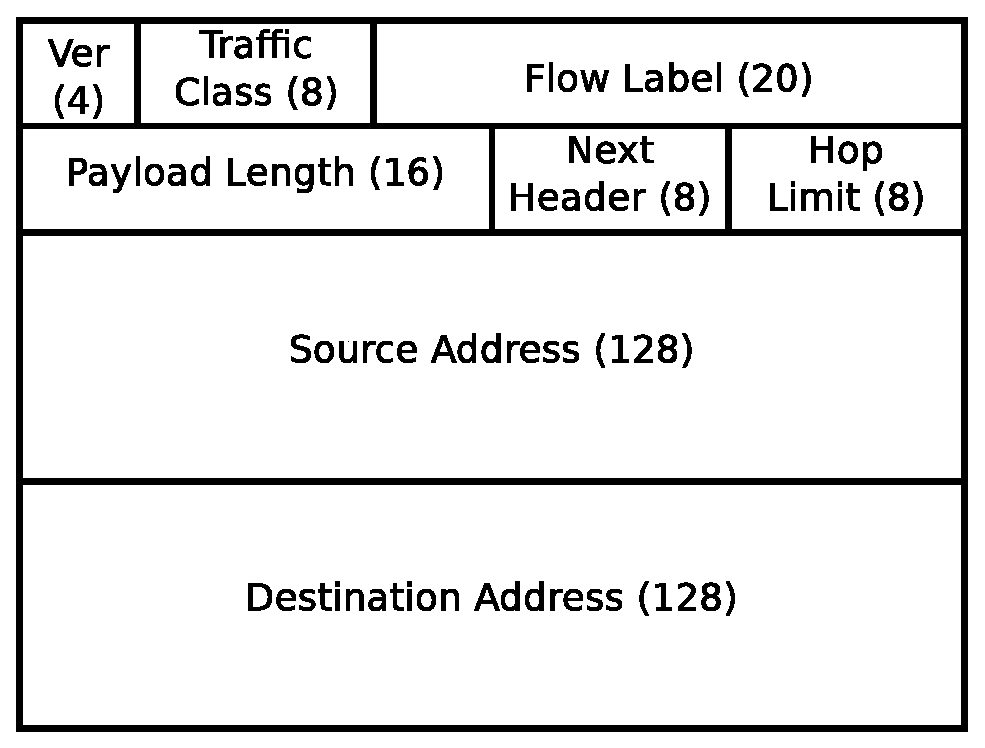
\includegraphics[width=4in]{IPv6_header}
\caption{L'en-tête IPv6}
\label{fig:IPv6}
\end{figure}

\begin{table}[htb]
\caption{Plages de valeurs pour le champ \texttt{DSCP}}
\centering
\begin{tabular}{|c|c|l|}
\hline\rowcolor[gray]{0.8}\color{black}
Plage & Valeurs & Règle d'assignation\\\hline
1 & xxxxx0 & Assignation par une norme de l'IANA\\\hline
2 & xxxx11 & Expérimentation/Usage local\\\hline
3 & xxxx01 & Expérimentation/Usage local (pourrait être jointe à la plage 1)\\\hline
\end{tabular}
\label{tab:RangesDSCP}
\end{table}

% On veut éviter que la figure et le tableau soient placés au-delà de la section courante.
% To prevent the figure and table from being positioned outside of the current section. 
\FloatBarrier


%%
%% OBJECTIFS DE RECHERCHE / RESEARCH OBJECTIVES
%%
\section{Objectifs de recherche}  % 0.5 page
Les objectifs de la recherche sont de concevoir un algorithme $O(n)$.


%%
%% PLAN DU MEMOIRE / THESIS OUTLINE
%%
\section{Plan du mémoire}  % 0.5 page

Voir la Figure~\ref{fig:Layers} pour plus de détails. 

\begin{figure}[htb]
\centering
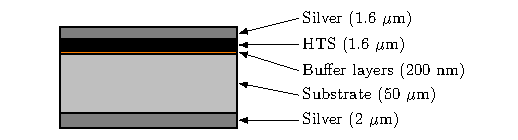
\includegraphics[width=4in]{demo_tikz}
\caption{Couches}
\label{fig:Layers}
\end{figure}


Un tableau : / A table:
\begin{table}[htb]
  \centering
  \caption{Constantes et variables du modèle analytique}
  \begin{tabular}{|c|l|}
    \hline\rowcolor[gray]{0.8}\color{black}
    Symbole         & Description\\\hline
    $\lambda$       & Taux d'arrivée moyen des requêtes de réservation de ressources\\\hline
    $\frac{1}{\mu}$ & Durée moyenne d'une session\\\hline
    $C$             & Capacité d'une cellule (nombre de sessions supportées)\\\hline
    $v_{moy}$       & Vitesse moyenne des MN dans le réseau d'accès\\\hline
    $L$             & Longueur d'un côté d'une cellule carrée\\\hline
    $n$             & Nombre moyen de MN dans une cellule\\\hline
    $\rho$          & Charge d'une cellule\\\hline
    $P_b$           & Probabilité de blocage d'une requête de réservation\\\hline
    $P_f$           & Probabilité d'interruption forcée d'une session\\\hline
    $P_c$           & Probabilité de compléter une session avec succès\\\hline
    $\Delta{}T$     & Délai de transmission\\\hline
  \end{tabular}
  \label{tab:Definitions}
\end{table}

La formule d'\mbox{Erlang-B}:
\begin{equation}
  P_b = \frac{\frac{\rho^C}{C!}}{\sum\limits_{x=0}^{C}\frac{\rho^x}{x!}}
  \label{eq:Pblock}
\end{equation}

Une autre équation : / Another equation:
\begin{equation}
  \begin{split}
    P_c &= (1 - P_b) \times (1 -  P_f)^N\\
        &= (1 - P_b)^{N+1}
  \end{split}
  \label{eq:ProbComplete}
\end{equation}

Enfin, l'expression suivante indique le moment à partir duquel les
réservations de ressources sont en place:
\begin{equation}
  \Delta{}T_{init} =
  \begin{cases}
    2\Delta{}T_{E2E} & \Delta{}T_{wan} > (\Delta{}T_{rad} + \Delta{}T_{net})\\
    \Delta{}T_{E2E} + 3(\Delta{}T_{rad} + \Delta{}T_{net}) & \text{sinon}
  \end{cases}
  \label{eq:InitCost}
\end{equation}

\paragraph{Le taux de paquets perdus} correspond au nombre de paquets
éliminés à cause d'une erreur de \emph{checksum} à un n\oe{}ud
quelconque ou d'une situation de congestion. Le taux de paquets perdus
pour un chemin est déterminé de la façon suivante:
\begin{equation}
  \label{eq:genPLR}
  PLR_P = 1 - \prod_{i=1}^N(1 - PLR_i)
\end{equation}

Toutefois, si les taux d'erreurs sont très faibles, comme c'est
généralement le cas pour des liens optiques, on peut approximer
$PLR_P$ de façon à le transformer en un paramètre additif:
\begin{equation}
  \label{eq:approxPLR}
  \begin{split}
    PLR_{L_1 \oplus L_2} &= 1 - (1 - PLR_1)(1 - PLR_2)\\
    &= 1 - (1 - PLR_2 - PLR_1 + \underbrace{PLR_1
      \times PLR_2}_\text{négligeable})\qquad PLR_1 \ll 1,
    PLR_2 \ll 1\\
    &\approx PLR_1 + PLR_2
  \end{split}
\end{equation}

\clearpage

Une courbe : / A curve:
\begin{figure}[htb]
\centering
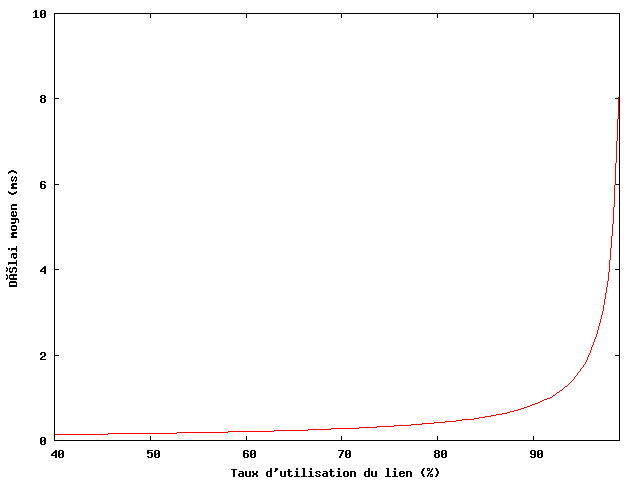
\includegraphics[width=5in]{LinkUsage}
\caption{Délai moyen en fonction du taux d'utilisation d'un lien}
\label{fig:LinkUse}
\end{figure}

\selectlanguage{english}
This paragraph is formatted by \LaTeX{} according to the standard rules of the
English language (\mbox{e.g.} hyphenation).
\selectlanguage{french}

L'arithmétique en virgule flottante peut entraîner des erreurs
d'approximation et il est important d'en être conscient
\cite{Rossi2011}.

De même, les calculs effectués sur une carte graphique (GPU) peuvent
introduire des erreurs d'approximation \cite{DeSantis2002, Cohen2006,
  Thorsson2014, Schirmer2012, Sakai2015, Electrical2006,
  Min2016, Massicotte2013, Kaliouby1987, Daintith2010, Haist2014, Kizza2013,
  Manasreh2011, Brydson1999, Boyce2002}.
       % Introduction au sujet de recherche.
\Chapter{REVUE DE LITTÉRATURE}\label{sec:RevLitt}
% Texte / Text.

\section{Robot logiciel développeur}

La définition de robot logiciel est «Agent intelligent programmé afin d'imiter les capacités d'un être humain dans un système informatique ou afin d'effectuer un ensemble de tâches prédéterminées de manière automatique.»~\cite{robot_logiciel_oqlf_2018} Les autres termes suggérés est «robot informatique» et «robot». Ainsi, un robot développeur, est un robot logiciel orienté au développement logiciel. En anglais, il pourrait être nommé un «DevBot».

La référence à l'aspect social d'un robot logiciel développeur est par exemple l'outillage aux développeurs autour d'un éditeur asynchrone en temps réel tel que CodeBuddy~\cite{10.1145/3287324.3293750} ou CodePilot~\cite{10.5555/1030453.1030540} dans leur développement collaboratif.

Le robot logiciel développeur idéal est «un développeur de logiciels artificiels qui est autonome, adaptable et possède des compétences techniques ainsi que sociales.»~\cite{8823643} Seulement les éléments des compétences techniques et sociales seront discutés dans ce mémoire, le tout orienté sur la plateforme ERPLibre avec de l'amélioration continue sur un réseau d'entraide.

\section{Génération de code}

Utiliser un générateur de code dans un contexte d'application web est efficace, l'auteur Uyanik.B, et a. de l'article «A template-based code generator for web applications»~\cite{SAHIN2020} obtient un gain de performance en temps de développement de 98.95\% et 0 bogue via le générateur de code.

Dans un autre projet de l'auteur Pichidtienthum.S et a. de l'article «»~\cite{9436754}, en ajoutant une interface LCNC sur un générateur de code sur Odoo, on obtient 20\% de réduction de temps pour le développement de module, puis des utilisateurs non développeur peuvent utiliser cet outil pour faire des modules. Ce projet est très similaire à celui expérimenté dans ce mémoire, sauf l'aspect de la rétro-ingénierie qui est manquante avec l'amélioration continue et la gestion d'un réseau d'entraide.

\section{Logiciel Libre et Open Source}

Actuellement, une méthode utilisée pour accélérer le développement, c'est le partage de bibliothèques : une fonctionnalité aurait déjà été programmé et le rendre accessible publiquement permet la réduction d’écriture du code pour réaliser une fonctionnalité souhaitée.

L’Open Source permet aussi de supporter l'interopérabilité~\cite{open_interop_2011}, c’est la capacité de différents logiciels d'interagir et communiquer efficacement entre eux de manière transparente et harmonieuse sans entraves ni obstacles, même s’ils ont été développés par différentes organisations.

D'ailleurs, comme le mentionne l'auteur Hertel.G et a. de l'article «Motivation of software developers in Open Source projects: an Internet-based survey of contributors to the Linux kernel»~\cite{HERTEL20031159}, un des facteurs de motivation important est la perception de l'indispensabilité de ses propres contributions dans une équipe, associé à une évaluation élevée des objectifs de l'équipe et un fort sentiment d'auto-efficacité personnelle. Le générateur de code ne doit pas remplacer l'utilisateur, il doit l'accompagner dans leur développement.

% \section{Logiciel Libre}
% Le logiciel libre entrave l’interopérabilité seulement pour les systèmes non compatibles avec la copyleft. Bien qu’elle prône la liberté du code, elle est restrictive.

% Cette restriction est nécessaire à la protection du développeur et de la communauté. 

\section{Sécurité}

«La morale de l'article~\cite{thompson_trusting_1984}, alors, est assez simple : il est impossible de fonctionner\footnote{D'utiliser et d'avoir confiance sur des technologies} sans faire confiance à quelqu'un. À moins que vous n'ayez écrit tout le code (et je veux dire TOUT le code) vous-même, vous devrez faire confiance à la sécurité d'une partie du processus de traitement du programme.»~\cite{discussion_reflection_trusting_2020} L'automate codeur doit apprendre à développer toute les étapes de programmation sur une machine.

Hors, s'il est nécessaire de faire confiance, peut-on faire confiance lorsqu'on observe des problème de compatibilité de licence libre~\cite{pfeiffer2022license}\cite{8667977}? Le développeur utilise des bibliothèques libres qui utilisent d'autre bibliothèques pas nécessairement libres et qui peuvent contenir des failles de sécurités~\cite{10.1145/3133956.3134048}, sans en être conscient. Le robot codeur doit ainsi être en mesure de faire du développement sur les bibliothèques utilisés.

«Cela suggère que tant que nous ne sommes pas en mesure de rétroconception\footnote{Faire de la rétro-ingénierie sur un développement.} et de contrôler pleinement la fonctionnalité des réseaux neuronaux, il existera un risque inhérent. Même si nous parvenons à résoudre le problème d'alignement et à rendre l'IA conviviale pour l'homme, les attaquants qui obtiennent un accès en écriture aux poids\footnote{Un poids est la valeur numérique d'une neurone dans un réseau de neurones.} pourront implanter leurs portes dérobées.»~\cite{discussion_reflection_trusting_ia_2023} L'automate doit être en mesure de comprendre le fonctionnement du logiciel pour l'étudier.

\section{Les complexités de développer ERP}
% TODO voir article erp en entreprise
% REF implantation d’un ERP en PME

Le développement d’une solution ERP doit supporter plusieurs niveaux~\cite{uqam_erp_benefice_2008} : 
\begin{enumerate}
    \item Évaluation des besoins;
    \item Préparation du projet;
    \begin{enumerate}
        \item Organisation du projet;
        \item Définir les objectifs;
        \item Créer un plan détaillé;
    \end{enumerate}
    \item Dessin d’affaires;
    \begin{enumerate}
        \item Analyser les processus d’affaires actuels;
        \item Maîtrise du système ERP;
        \item Revue des processus;
    \end{enumerate}
    \item Réalisation;
    \begin{enumerate}
        \item Développement technique;
        \item Étude pilote;
    \end{enumerate}
    \item Préparation finale;
    \begin{enumerate}
        \item Réglages et tests;
        \item Éduquer et former la masse critique;
    \end{enumerate}
    \item Mise en production et support;
    \begin{enumerate}
        \item Déploiement des modules ERP;
        \item Améliorer et élargir les systèmes ERP de façon continue;
    \end{enumerate}
\end{enumerate}

Autour de ça, il faut mettre en place une gestion du changement et adapter le développement des affaires.

Plusieurs de ces étapes ne sont pas prises au sérieux, tel que le financement. De plus, l’implantation se fait sur une longue période de temps.

Dans Odoo, le nombre de modules augmente avec le temps et diffère entre les versions, une recherche fastidieuse doit être effectuée pour réduire le temps de développement et à éviter de réinventer la roue.

Il faut adapter les processus des organisations aux fonctionnalités existantes, sinon il est trop coûteux de tout recréer selon les processus de l’entreprise.

En plus de suivre toutes ces étapes, il faut mettre en place une pérennité pour l’amélioration continue sur le projet, cela rend le processus lourd en plus de durer dans le temps.


\section{Logiciel no-code / low-code}

Logiciel no-code / low-code = LCNC

Basé sur des templates de code et une interface qui, au besoin, permet la configuration par du code.

C’est un concept qui permet à l’utilisateur de développer une plateforme en utilisant pas ou peu de code.

% TODO REF A. C. Bock, U. Frank: Low-Code Platform, Bus Inf Syst Eng 63(6):733–740 (2021)
% TODO REF Supporting the understanding and comparison of low-code development platforms

Besoin de : 
\begin{enumerate}
    \item Aspect général;
    \begin{enumerate}
        \item Gestion des rôles et permissions par des groupes utilisateurs ou individuelle;
        \item Mécanisme de déploiement et exportation;
    \end{enumerate}
    \item Perspective d’intéraction;
    \begin{enumerate}
        \item Mécanisme pour changer le design de l’interface utilisateur;
        \item Mécanisme pour coupler l’interface à un modèle et un contrôleur (MVC);
        \item Mécanisme pour faire le rendu visuel sur différents types d’appareils;
    \end{enumerate}
    \item Perspective dynamique;
    \begin{enumerate}
        \item Gestion des processus du système et de la machine;
        \item Composantes de modélisation de processus conceptuel;
        \item Système de gestion des états et des transitions;
    \end{enumerate}
    \item Perspective fonctionnelle;
    \begin{enumerate}
        \item Mécanisme de spécification fonctionnel de base;
        \item Générateur d’algorithme;
        \item Générateur de code de composantes;
        \item Mécanisme d’accès à des API externe;
    \end{enumerate}
    \item Perspective statique;
    \begin{enumerate}
        \item Composante de conception d’un modèle de données;
        \item Composante pour spécifier des structures de données;
        \item Gestion de base de données interne;
        \item Gestion de base de données externes par API;
    \end{enumerate}
\end{enumerate}

Pour supporter une plateforme LCNC :
\begin{enumerate}
    \item Bases de données;
    \item Services externes;
    \item Gestion des modèles de données;
    \item Plateforme collaborative;
    \item Service infonuage (déploiement, audit de performance, gestion des erreurs/traces/événements, gestion des versions);
    \item Générateur de code;
    \item Compilateur et optimiseur de code;
    \item Modeleur d’application;
    \begin{enumerate}
        \item Widget;
        \item Connecteur;
        \item Processus de logique métier;
        \item Capacité de «drag and drop»;
        \item Modèle de données;
        \item Règles de sécurité;
    \end{enumerate}
\end{enumerate}
Critère de qualité d’une plateforme LCNC :
\begin{enumerate}
    \item GUI;
    \item Interoperability support entre services externes et base de données;
    \item Support de la sécurité;
    \item Support d’une plateforme collaborative;
    \item Support sur la réusabilité, pouvoir répété l’utilisation d’une composante dans différents contextes;
    \item Support de la capacité d’un système à maintenir ou à améliorer ses performances;
    \item Mécanisme de spécification de logique du développement des affaires;
    \item Logiciel pour construire des mécanismes;
    \item Support au déploiement;
\end{enumerate}

% \section{Dev ops}
% Démontrer outil
% TODO image dev ops

% La partie générateur de code répond seulement au besoin création de code du dev ops.

\section{Création d’une communauté}

\subsection{Communication non violente}

Réduire les frictions entre les participants du réseau d’entraide. C’est avec la mise en place d’une méthode de communication non violente~\footnote{\url{https://fr.wikipedia.org/wiki/Communication_non_violente}} formalisée par Marshall B. Rosenberg, voir Figure~\ref{fig:communication_non_violente}.

\begin{figure}[htb]
\centering
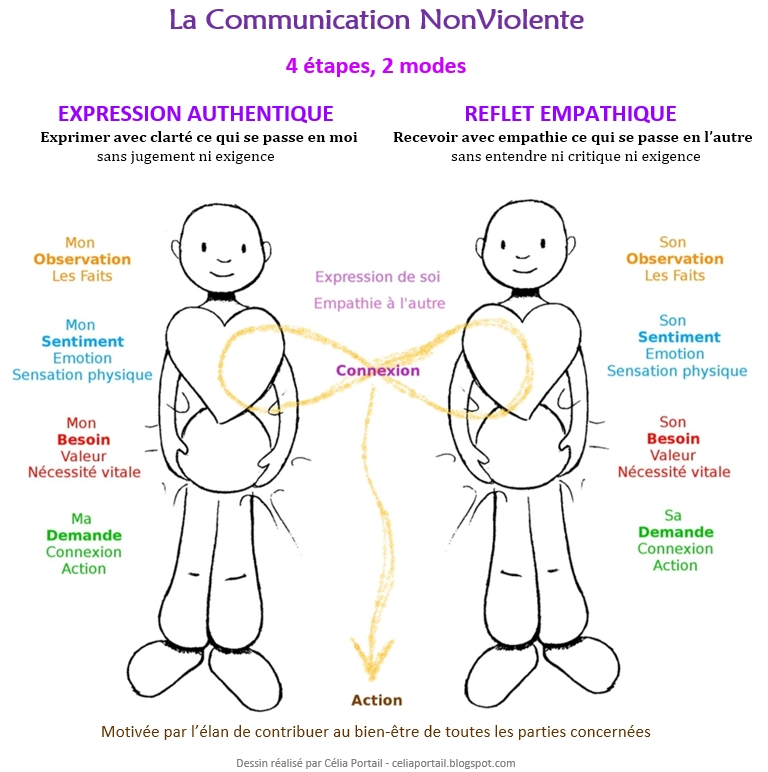
\includegraphics[width=4in]{OSBD_en_CNV.jpg}
\caption{Communication non violente en 4 étapes et 2 modes}
\label{fig:communication_non_violente}
\end{figure}

\subsection{Guide construire une communauté Open Source}
Guide en 4 sections avec des titres indicateurs d’orientation pour un gestionnaire de communauté :

\begin{enumerate}
    \item Mise en place de votre projet pour le succès;
    \item Cultiver votre communauté;
    \item Résoudre les conflits;
    % \item La communauté est le coeur ❤️ de l’open source.
    % \item La communauté est le coeur ❤ de l’open source.
    \item La communauté est le coeur de l’open source.
\end{enumerate}

Il faut :
\begin{enumerate}
    \item rédiger un code de conduite;
    \item proposer la contribution directement sur le projet.
\end{enumerate}
% TODO supporter les autres pages https://opensource.guide/fr/metrics/

Ils n'intègrent ni les aspects de génie industriel qui est vulgarisé avec le guide fusée et ni les critères éthiques de GNU concernant l’hébergement de logiciel.

\subsection{Guide fusée}

Un guide en 7 étapes~\ref{fig:guide_fusee} pour les gestionnaires de projet. Il vous permet de démarrer un projet rapidement qui nécessite une équipe de personnes pour les rendre efficaces dans la réalisation de leurs participations dans le réseau d’entraide.

% REF guide fusée polylabac/cimarlab

\begin{figure}[htb]
\centering
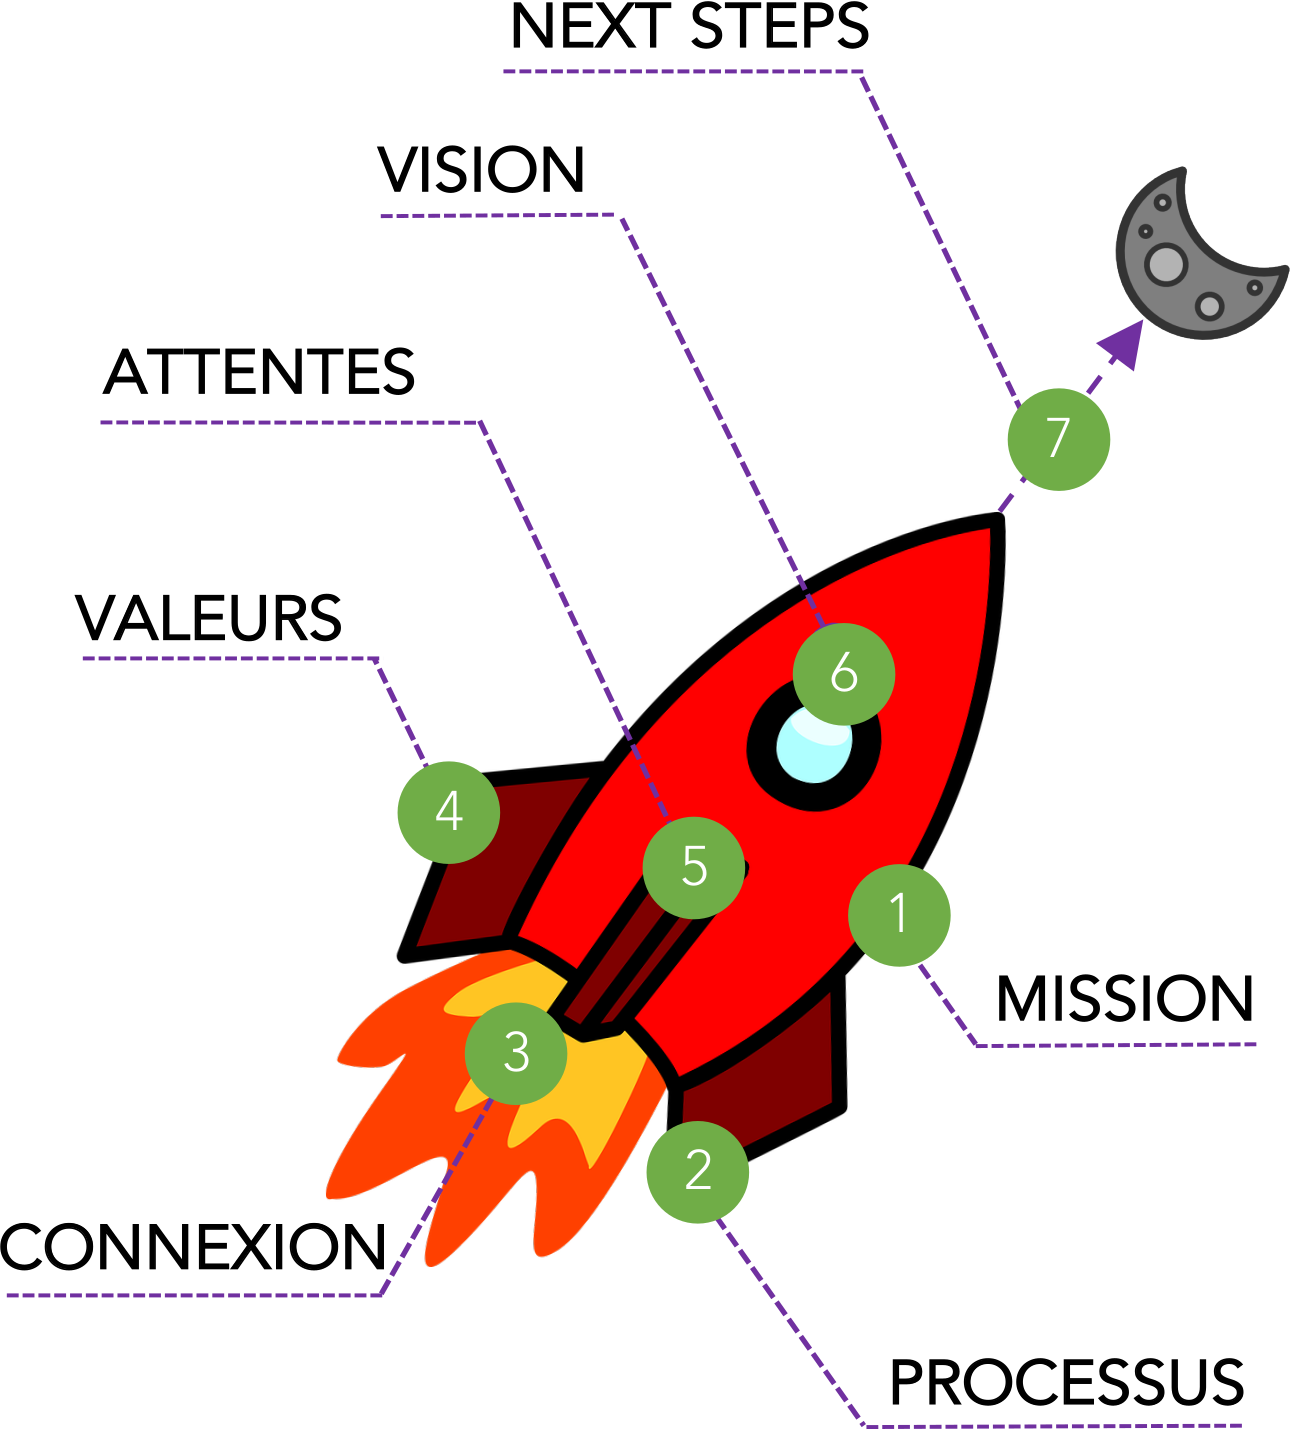
\includegraphics[width=4in]{guide_fusee_definition.png}
\caption{Guide fusée de CimarLab}
\label{fig:guide_fusee}
\end{figure}

\subsection{Critères éthiques de GNU concernant l'hébergement de logiciel}

La licence AGPLv3 n’est pas toujours bien respectée~\cite{violation_libre_2017}.

Les critères éthiques concernant l'hébergement de logiciel~\cite{gnu_critere_hebergement_2022} doivent être accessibles sur les projets de réseau d’entraide. Un guide avec des critères mesurables pour les services destinées à tous ceux qui veulent utiliser un service pour héberger publiquement du code source libre, ainsi qu'éventuellement des programmes exécutables. Ces critères se concentrent sur la protection de la vie privée, le fonctionnement sans JavaScript non libre\footnote{\url{https://www.fsf.org/campaigns/freejs}} , la compatibilité avec les licences à copyleft et leur philosophie, et l'absence de discrimination contre les utilisateurs, quels qu'ils soient.  Les questions à répondre : 

\begin{enumerate}
    \item Est-ce que l'hébergeur fournit l'accès au code source des programmes qu'il héberge?
    \item Est-ce que l'hébergeur permet la redistribution des copies des programmes qu'il héberge?
    \item Est-ce que l'hébergeur permet aux utilisateurs d'apporter des modifications aux programmes qu'il héberge et de les partager avec la communauté?
    \item Est-ce que l'hébergeur impose des restrictions sur l'utilisation ou la redistribution des programmes qu'il héberge?
    \item Est-ce que l'hébergeur respecte les licences de logiciels libres et les droits d'auteur associés aux programmes qu'il héberge?
    \item Est-ce que l'hébergeur fournit des informations sur les licences de logiciels libres et les droits d'auteur associés aux programmes qu'il héberge?
    \item Est-ce que l'hébergeur respecte la vie privée et la sécurité des utilisateurs des programmes qu'il héberge?
    \item Est-ce que l'hébergeur fournit un support et une assistance adéquats aux utilisateurs des programmes qu'il héberge?
\end{enumerate}

\section{Poïèse}

\subsection{Définition de la poïèse}

La poïèse (ou poïesis) est un terme d'origine grecque qui désigne le processus créatif de fabrication, de production ou de création. Il est souvent utilisé dans le contexte de l'art et de la littérature pour décrire le processus de création d'une œuvre, que ce soit un poème, une pièce de théâtre, un roman ou une peinture.

Dans ce contexte, la poïèse est considérée comme un processus actif et dynamique, impliquant l'imagination, l'inspiration, la créativité et la maîtrise technique. Elle implique souvent un certain niveau d'engagement personnel et émotionnel de la part de l'artiste\label{poiese_artise} ou du créateur.

En dehors de l'art, le terme poïèse peut également être utilisé pour décrire tout processus de création ou de production, y compris dans des domaines tels que la science, la technologie ou l'industrie.

Les termes «Allopoïèse», «Autopoïèse», «Sympoïèse» ont été inventés pour décrire des phénomènes biologiques, hors dans ce mémoire, ils ont été adaptés pour un contexte technologique.

\subsection{Allopoïèse}

Un système qui développe\footnote{production/fabrication : Utiliser sans limitation, Modifier pour adapter, Étudier pour comprendre le fonctionnement et Copier pour reproduire.} quelques choses avec des composantes externes.

«L'allopoïèse est le processus par lequel un système produit quelque chose qui n'est pas le système lui-même. Ceci est le contraire de l'autopoïèse.[...] La plupart des processus de production industrielle sont allopoïétiques : une chaîne de montage peut produire des voitures mais pas les machines utilisées dans cette forme de production. [...] La reproduction n'est pas une auto-production.»~\cite{wiki_allopoiesis_2018}~\cite{vuc_allopoiesis_2018}


% «une définition qui est proche de celle d’une machine abstraite et qui décrit la machine comme autopoïétique, autoproductrice d’elle-même et reproduisant en permanence ses composantes tel un système sans input ni output. Varella développe assez loin cette théorie. Il oppose dans sa conception, l’autopoïèse qu’il rapporte essentiellement aux êtres vivants biologiques, à une allopoïèse où la machine va chercher ses composantes à l’extérieur d’elle-même. En fait, dans son concept d’allopoïèse il range les systèmes sociaux, les machines techniques et, pour finir, tous les systèmes machiniques qui ne sont pas des systèmes vivants.»
% «Les machines allopoïétiques se trouvent toujours en adjacence à des machines autopoïétiques et il faut donc prendre en considération les agencements qui les font vivre ensemble.»
% Citer ce document / Cite this document :
% Guattari Félix. À propos des machines. In: Chimères. Revue des schizoanalyses, N°19, printemps 1993. pp. 85-96 ;
% doi : https://doi.org/10.3406/chime.1993.1881
% https://www.persee.fr/doc/chime_0986-6035_1993_num_19_1_1881


\subsection{Autopoïèse}

Un système qui se développe par soi même avec seulement ses composantes internes.

«L'autopoïèse est la propriété d'un système de se produire lui-même, en permanence et en interaction avec son environnement, et ainsi de maintenir son organisation (structure) malgré son changement de composants (matériaux) et d'informations (données).[...]le maintien de sa propre organisation (auto-production)»~\cite{wiki_autopoiesis_2022}.

Le maintien de sa propre organisation signifie l'auto-production, voir exemple illustratif auto-reproducteur~\ref{exemple_illustratif_auto_reproducteur}.

Un système est de l'autopoïèse~\cite{tatsuya_computational_autopoiesis_2000} dans le contexte qu'il est : 
\begin{enumerate}
    \item \textbf{Autonome} : il doit être capable d'apporter des changements variés pour maintenir son organisation;
    \item \textbf{Individuel} : il doit être indépendant dans sa définition, par sa prise de décision par rapport aux observateurs externes, en reproduisant à répétition et en maintenant son organisation;
    \item \textbf{Connaissant et établis ses limites} : il doit être capable d'établir ses limites dans son processus de reproduction par lui même sans se faire affecter des limites établis par les observateurs externes;
    \item \textbf{Absent d'entrant et de sortant} : Les stimulis externes doivent être interprété dans un contexte d'observation pour en retirer de l'amélioration continue, elles ne doivent pas impacter la maintenance de l'organisation directement, mais son évolution doit en prendre compte.
\end{enumerate}

Le concept de vue sur les entrants et sortants d'un système est une perception des observateurs externes et ne clarifie pas l'organisation ou les opérations de production du système. 

% TODO à valider : Ainsi, le système va opérer sans s'ajuster lui-même en rapport avec son état et le stimulis externe.

% TODO Alors comment fait-il pour se produire lui même en interaction avec son environnement s'il n'a pas d'entrant et sortant?

La conception d'un système autopoïèse\cite{tatsuya_computational_autopoiesis_2000} devrait comporter les points suivants : 

\begin{enumerate}
    \item Les composantes du système sont déterminés par les opérations du système;
    \item Les opérations du système sont produites avant les conditions initiales;
    \item Les opérations du système sont seulement exécutées pour leur propre réussite et non pour réaliser la production d'un produit;
    \item Dans les opérations du système, ce qui se passe à l'intérieur du système est clairement différent des jugements des observateurs externes.
\end{enumerate}

% TODO La Technopoïèse doit être différent de l'autopoïèse, bien qu'il doit être autonome dans son évolution, il doit suivre des principes moraux et respecter des règles de société.

%  L'autopoïèse s'applique aussi à l'être humain, tant en sociologie\footnote{\url{https://fr.wikipedia.org/wiki/Sociologie}}, la science cognitive\footnote{\url{https://fr.wikipedia.org/wiki/Sciences_cognitives}}, la philosophie\footnote{\url{https://fr.wikipedia.org/wiki/Philosophie}} et la psychopathologie\footnote{\url{https://fr.wikipedia.org/wiki/Psychopathologie}}.

Appliquer l'autopoïèse sur un système est de forcer un changement de point de vue vers l'intérieur du système, puisque l'extérieur est matière à interprétation par la distinction de son environnement. En sciences naturelles, ce changement de point de vue est difficilement acceptable puisque le point de vue est fait par des observateurs externes.

Des modèles mathématiques sont expliqués dans l'article~\cite{tatsuya_computational_autopoiesis_2000} tel un système de réparation du métabolisme ((M,R) systems), introduit par Rosen, pour démontrer le «Quasi-Autopoietic Systems».
Puis il y a des modèles d'apprentissage automatique qui ont été inspirés de l'autopoïèse pour effectuer des tâches de reconnaissance de formes. Pour pouvoir représenter l'autopoïèse en mathématique ou en modèle informatique, il est nécessaire de trouver un mécanisme d'un système qui crée son espace avec ses limites et son environnement, par soi-même.

% TODO documentation intéressante : https://www.researchgate.net/publication/228784157_A_Computational_Aspect_of_Autopoiesis

\subsection{Sympoïèse}

Un système qui développe en collectivité. Caractéristique d'une technologie qui fait de la poïèse.

La sympoïèse est un concept utilisée en écologie et en théorie des systèmes pour décrire les processus de production collective et collaborative dans les écosystèmes. Elle se distingue de l'autopoïèse, qui est le processus par lequel un système produit et reproduit ses propres composants de manière autonome. Par exemple, les coraux sont des collectifs d'organismes en interaction qui produisent des structures complexes telles que des récifs, qui ont des effets bénéfiques sur l'écosystème dans son ensemble.

«La nature est une puissance d’engendrement qui surgit et s’autoproduit. Donna Haraway a récemment proposé de remplacer le concept "d’autoproduction" par celui de "sympoïèse" qui désigne la coproduction du milieu par des espèces en interrelations plutôt que l’activité autonome de certains organismes isolés.»~\cite{guillibert:tel-02929676}

\subsection{Technopoïèse}

Un système technologique qui développe. Caractéristique d'une technologie qui fait de la poïèse.

% Un système technologique qui travaille pour la poïèse en mettant en place plusieurs caractéristiques, par exemple : l'«Allo» et l'«Auto».

La technologie est là pour assister l'utilisateur et l'accompagner dans l'évolution de celle-ci. «Parce que l’appareil prend place entre la manifestation de l’œuvre et le travail de l’artiste en les découplant, en leur imposant une langue intermédiaire qui code puis décode. L’artiste produit des lignes de code, que la technologie intègre pour fournir à l’œuvre la source de sa manifestation : elle sépare ontologiquement\footnote{Une ontologie est une représentation formelle et explicite de la connaissance d'un domaine, qui spécifie les concepts, les relations et les entités qui existent dans ce domaine et comment ils sont interconnectés.} le travail de l’un et son résultat dans l’autre.»~\cite{artiste_techno_conf_2012} L'artiste~\footnote{Voir l'artiste de la «Définition de la poïèse»~\ref{poiese_artise}} ici signifie un programmeur informatique dans un processus créatif de fabrication, de production ou de création sur des technologies.

Pour éviter que la machine prend le dessus, il faut l'orienter vers la technopoïèse. «Si la technologie est un médium parasite, alors ne suffit-il pas de compter sur la charge poïétique du médium primaire, pour conserver à la poïèse ses caractères nécessaires – et imaginer l’art technologique comme un art d’abord, agrémenté, partiellement seulement, de technologie?»~\cite{artiste_techno_conf_2012} % Cette machine doit être libre pour respecter l'humain. % TODO référence machine libre respect humain

%«Our main claim in this study is to underline that the biopoetic process organizing technopoiesis involves at least four levels, with emergences and constrains between the levels. Furthermore, we see technopoiesis as the dynamics between these four levels based on mechanisms expressing the relation between biology, poetics and external representations that cognitively and socio-culturally ground the evolution of technology.»~\cite{10553_41343}

La relation entre la sympoïèse et la technopoïèse permettrait de concevoir des technologies plus durables et écologiquement responsables, qui favorisent la production collective et collaborative dans les écosystèmes.

Ainsi, le terme «technopoïèse» fait référence à la capacité de l'humanité à créer et à façonner la technologie pour répondre à ses besoins et à ses désirs. 

\subsection{Auto-technopoïèse}

% TODO source chatgpt

% L'auto-technopoïèse étend cette idée, de la technopoïèse, en suggérant que les systèmes technologiques peuvent devenir autonomes et se réguler eux-mêmes sans l'intervention humaine.

L'auto-technopoïèse est un concept qui décrit la capacité des systèmes technologiques à s'auto-organiser et à s'auto-réguler. Plus précisément, l'auto-technopoïèse se réfère à la capacité des systèmes technologiques à maintenir leur propre structure, leur fonctionnement et leur évolution, en utilisant des mécanismes internes de régulation et d'adaptation.

% Le terme "technopoïèse" fait référence à la capacité de l'humanité à créer et à façonner la technologie pour répondre à ses besoins et à ses désirs. L'auto-technopoïèse étend cette idée en suggérant que les systèmes technologiques peuvent devenir autonomes et se réguler eux-mêmes sans l'intervention humaine.

% Un exemple d'auto-technopoïèse est l'Internet, qui est un système complexe de réseaux informatiques interconnectés à l'échelle mondiale. L'Internet est capable de s'auto-réguler et de s'adapter à des changements dans son environnement, tels que l'augmentation du trafic de données ou les pannes de serveurs. Cela est rendu possible grâce à des mécanismes internes de régulation, tels que les protocoles de communication standardisés et les systèmes de routage dynamique.

% En résumé, l'auto-technopoïèse est un concept qui décrit la capacité des systèmes technologiques à s'auto-organiser et à s'auto-réguler. Cette capacité est de plus en plus importante à mesure que les systèmes technologiques deviennent plus complexes et interconnectés.

Pour faire des améliorations technologiques dans la société, sur des réseaux d'entraide, il faut orienter l'auto-technopoïèse dans de la R\&D~\cite{innovation_complex_social_system_2010} orienté aux besoins technologiques dans la gestion de cas d'urgence humanitaire, par exemple le «mouvement des villes en transition»~\cite{MOUV_063_0130}\footnote{\url{https://fr.wikipedia.org/wiki/Ville_en_transition}}, en lien avec la sympoïèse.

% https://transitionlibre.ca

% Référence : 
% Teubner, G. (1993). Autopoietic law: A new approach to law and society. Walter de Gruyter.
% Luhmann, N. (1986). The autopoiesis of social systems. John Wiley & Sons.
% Castells, M. (1996). The rise of the network society. Blackwell Publishers.
% Ahrweiler, P. (2012). Innovation in complex social systems. Routledge.
  % Revue de littérature / Literature review
\Chapter{PREMIER THÈME / FIRST THEME}\label{sec:Theme1}
Texte / Text.
             % Premier thème (Doctorat) ou "Détails de la Solution" (Maîtrise) / First topic (PhD) or "Details of the Solution" (Master's).
\Chapter{SECOND THÈME / SECOND THEME}\label{sec:Theme2}
Texte / Text.
             % Second thème (Doctorat) ou "Résultats théoriques et expérimentaux" (Maîtrise) / Second theme (PhD) or "Theoretical and experimental results" (Master's)
\Chapter{TROISIÈME THÈME AVEC UN TITRE TRÈS LONG QUI S'ÉTEND SUR DEUX LIGNES / THIRD THEME WITH A VERY LONG TITLE THAT EXTENDS ON TWO LINES}\label{sec:Theme3}

Lorem ipsum dolor sit amet, non faucibus ut, ante integer tristique odio
vitae turpis in. Euismod ullamcorper urna eget sollicitudin consectetuer,
dolor a. Ridiculus volutpat fusce, montes ipsum placerat, eu malesuada
maecenas a odio per, est pellentesque integer auctor sed ut sed, lectus
sodales orci ornare. Donec neque turpis vehicula. Duis vel sapien nec massa
lobortis nonummy. Feugiat ultrices urna mauris.

Potenti erat molestie ridiculus placerat, viverra ut felis porttitor,
rhoncus accumsan non, dui magna quam justo, ultrices massa ut phasellus
donec viverra mauris. Mauris a, dictumst risus a ornare velit nulla
ultricies, neque leo pellentesque, sit sed et suscipit excepteur
aenean. Venenatis sodales, odio nostra in id nobis scelerisque, venenatis
sociosqu gravida blandit orci pellentesque, tincidunt velit sed elementum
lacus pretium nunc, aenean vel dui id. Elit placerat id dui nunc mollis,
diam sapien porta, ipsam elit magna imperdiet amet, erat feugiat, et eros
morbi feugiat velit fringilla. Lacinia phasellus lacinia magna nunc sed, a
rhoncus, sem eget, dui aliquam sit sed leo beatae non, quisque justo
dignissim.

Torquent curabitur magnis nullam viverra scelerisque, per lacus pellentesque
vivamus, mauris aliquam sem lacus vivamus nullam porta. Vivamus donec
maecenas nunc orci massa, orci neque luctus leo non, mauris quis metus
sagittis. Voluptatibus gravida interdum. Magna duis nulla odio lacus fugiat
non. Magna fusce nunc, eget pellentesque nec. Imperdiet non magna
sollicitudin pellentesque, fusce erat interdum diam tellus vel, vitae
iaculis lectus varius suspendisse. Ac vel a in semper tellus, lobortis sed,
ipsum volutpat. Mauris a nunc aliquam metus nec, eu et id risus, diam
integer molestie suspendisse, sed wisi. Metus sed justo sodales sapien
molestie, suspendisse sem viverra ac proin, lorem luctus at tellus, velit mi
morbi orci in vestibulum, dignissim urna ornare id donec. Suspendisse non
enim euismod odio elit mauris, consectetuer pellentesque faucibus velit ante
lacinia sed.

Et dui erat. Wisi lorem eleifend cursus do donec, sed vel fermentum nec, a a
in pharetra. Ultricies risus, eget habitasse in, consectetuer metus in
auctor ac pellentesque curabitur, pulvinar aliquet eget. Mattis eget
venenatis dolor, nunc sem sed massa, urna scelerisque a magnis, neque elit
nec aliquam nonummy ac accusantium. Id vivamus nunc, erat justo tellus,
scelerisque habitasse accumsan tellus, pede sem vestibulum velit in et
eleifend. Nulla massa aenean integer dui. Suscipit nunc purus, rutrum velit,
mi torquent elementum in tincidunt. Maecenas nulla integer fringilla dapibus
tellus sit, enim amet magna eu erat, libero consectetuer nisl sapien, in
ultricies neque arcu sodales sagittis.

Lorem ipsum dolor sit amet, non faucibus ut, ante integer tristique odio
vitae turpis in. Euismod ullamcorper urna eget sollicitudin consectetuer,
dolor a. Ridiculus volutpat fusce, montes ipsum placerat, eu malesuada
maecenas a odio per, est pellentesque integer auctor sed ut sed, lectus
sodales orci ornare. Donec neque turpis vehicula. Duis vel sapien nec massa
lobortis nonummy. Feugiat ultrices urna mauris.

Potenti erat molestie ridiculus placerat, viverra ut felis porttitor,
rhoncus accumsan non, dui magna quam justo, ultrices massa ut phasellus
donec viverra mauris. Mauris a, dictumst risus a ornare velit nulla
ultricies, neque leo pellentesque, sit sed et suscipit excepteur
aenean. Venenatis sodales, odio nostra in id nobis scelerisque, venenatis
sociosqu gravida blandit orci pellentesque, tincidunt velit sed elementum
lacus pretium nunc, aenean vel dui id. Elit placerat id dui nunc mollis,
diam sapien porta, ipsam elit magna imperdiet amet, erat feugiat, et eros
morbi feugiat velit fringilla. Lacinia phasellus lacinia magna nunc sed, a
rhoncus, sem eget, dui aliquam sit sed leo beatae non, quisque justo
dignissim.

Torquent curabitur magnis nullam viverra scelerisque, per lacus pellentesque
vivamus, mauris aliquam sem lacus vivamus nullam porta. Vivamus donec
maecenas nunc orci massa, orci neque luctus leo non, mauris quis metus
sagittis. Voluptatibus gravida interdum. Magna duis nulla odio lacus fugiat
non. Magna fusce nunc, eget pellentesque nec. Imperdiet non magna
sollicitudin pellentesque, fusce erat interdum diam tellus vel, vitae
iaculis lectus varius suspendisse. Ac vel a in semper tellus, lobortis sed,
ipsum volutpat. Mauris a nunc aliquam metus nec, eu et id risus, diam
integer molestie suspendisse, sed wisi. Metus sed justo sodales sapien
molestie, suspendisse sem viverra ac proin, lorem luctus at tellus, velit mi
morbi orci in vestibulum, dignissim urna ornare id donec. Suspendisse non
enim euismod odio elit mauris, consectetuer pellentesque faucibus velit ante
lacinia sed.

Et dui erat. Wisi lorem eleifend cursus do donec, sed vel fermentum nec, a a
in pharetra. Ultricies risus, eget habitasse in, consectetuer metus in
auctor ac pellentesque curabitur, pulvinar aliquet eget. Mattis eget
venenatis dolor, nunc sem sed massa, urna scelerisque a magnis, neque elit
nec aliquam nonummy ac accusantium. Id vivamus nunc, erat justo tellus,
scelerisque habitasse accumsan tellus, pede sem vestibulum velit in et
eleifend. Nulla massa aenean integer dui. Suscipit nunc purus, rutrum velit,
mi torquent elementum in tincidunt. Maecenas nulla integer fringilla dapibus
tellus sit, enim amet magna eu erat, libero consectetuer nisl sapien, in
ultricies neque arcu sodales sagittis.

             % Troisième thème (Doctorat) ou effacez ce fichier si vous êtes à la Maîtrise / Third topic (PhD) or delete this file if you are in the Master's program
\Chapter{CONCLUSION}\label{sec:Conclusion}
% Texte / Text.

%%
%%  SYNTHESE DES TRAVAUX / SUMMARY OF WORKS
%%
\section{Synthèse des travaux}
% Texte / Text.
Les résultats obtenus ont permis d’atteindre en tout ou en partie l’ensemble des sous-objectifs énoncés dans le chapitre~\ref{chapitre_methode}.%, voir Tableau~\ref{tab:synthese_travaux}.

\subsection{Projet Accorderie}
% TODO synthèse
La migration de la base de données a été réussie, mais elle est encore à ce jour en adaptation vers un modèle Odoo plus intégré au ERP. Les efforts ont été mis pour la création d’une interface utilisateur avec des technologies qui n’étaient pas à la base supportées dans Odoo.

\subsection{Projet Portail CEPPP}
% Synthèse
La signification que le nombre de lignes de XML aurait diminué, c’est que l’automate génère de base toutes les vues de tous les champs. Au moment de la ré-ingénierie, il y a eu beaucoup de nettoyage et de données XML effacées. Cependant, le développeur va mettre plus de code Python pour développer des logiques qui ne sont pas supportés par l’automate. Le Javascript ajouté sert à supporter les dates dans le portail. L’ajout de CSV sert pour l’ajout de permissions et rôles pour l’anonymisation.

Après la première migration par l’extraction du modèle de données par PHP, le client a pu testé la plateforme pour avoir une idée à quoi ressemblerait l’utilisation dans l’espace administration de leur modèle de données et ils ont fait des demandes de changement. Une analyse a été effectuée, nous avons utilisé le générateur de code pour générer les vues portails et fait une ré-ingénierie manuelle du modèle et des vues pour obtenir le résultat désiré. Une des fonctionnalités implémentés est l’anonymisation des données pour certains groupes d’utilisateurs, pour pouvoir visualiser des données sans avoir d’information personnelle sur le patient.




%%
%%  LIMITATIONS
%%
\section{Limitations de la solution proposée}\label{sec:Limitations}
% TODO dire en quoi ce que tu as fait améliore l’état de l’art décrit dans la littérature SYNTHÈSE
% TODO décrire les limitations/faiblesses de ce que tu as produit comme logiciel/résultats LIMITATION

\subsection{Couverture des tests}
% TODO limitation
Les tests devraient couvrir 100\% du code, cependant la couverture est de 84\% pour 3 raisons :

\begin{enumerate}
    \item Il y a du code fonctionnel non testé, il manque des tests;
    \item Il y a du code désuet qu’il faut nettoyer ou refactoriser;
    \item La gestion des erreurs n’est pas couverte, il faudrait les ignorer dans le test de couverture et faire des tests unitaires qui valide la gestion des erreurs.
\end{enumerate}


%%
%%  AMELIORATIONS FUTURES / FUTURE RESEARCH
%%
\section{Améliorations futures}
% Texte / Text.
% TODO dire ce qui doit être fait pour que les aspects d’utilisabilité de ton logiciel en terme de communauté, de libre, etc soient complets.

% TODO parler de la sympoïèse comme étant la suite sur la partie communautaire et la distribution de système


\subsection{Amélioration du générateur code}
% TODO amélioration future
Il faut intégrer la génération de code à l’intérieur des instances clientes dans l’objectif qu’ils soient accessibles de son gestionnaire de déploiement pour y ajouter les nouvelles fonctionnalités, démarrer la mise à jour, les tests, les améliorations, la migration, importation. Les instances clientes devraient proposer aux clients via les interfaces 

% Intégration de plusieurs types de réseaux de neurones accessibles librement, il doit être compatible avec le libre.

% Il faut suggérer aux clients des améliorations et de communiquer avec leurs gestionnaires de déploiements.

% Un générateur de code a été créé. L’embryon est créé, il faut terminer sa génération du générateur de code. Les déviances sont déjà créées

Une fois que le générateur de code aura atteint 100\% d’auto-génération, il restera limité à produire que les fonctionnalités qu’il utilise. Donc s’auto-générer fait office de test. Il faut faire des tests pour les fonctionnalités qu’il n’utilise pas (ou les combinaisons non utilisés) pour se reproduire. Il reste à auto-générer toutes ses techniques dans des modules qui font de l'héritage sur le générateur de code.

% Ajout de la génération de test de base, génération de documentation, mise à jour, migration lors d’une mise à jour sur les données, migration d’une mise à jour de la plateforme.

\subsubsection{Amélioration de l’architecture}
% TODO amélioration future
Parallélisation de tout le code tout le temps lorsque possible.

Automatisation de la configuration pour le déverminage, automatiser la détection des anomalies, améliorer l’interface no-code pour pouvoir accomplir les mêmes étapes que le mode de paramétrisation «Code hook». Supporter de nouvelles architectures dans la génération de code comme des applications Cordova pour le support mobile natif, des extensions Javascript dans Gnome Shell pour étendre les fonctionnalités du ERP directement sur le bureau d’un ordinateur sans passer par un navigateur web, générer des scripts de développement dans le projet ERPLibre qui ne dépendant pas d’Odoo, ou même supporter des applications embarqués.

De plus, il serait pertinent de supporter d’autres ERP externe comme NextERP ou Tryton qui sont des solutions libres. Cela va permettre la migration entre ERP des fonctionnalités et encourager l’utilisateur à prendre une solution entièrement AGPLv3 avec une communauté qui le supporte dans cette philosophie.

Problème d’extraction, il était dans le générateur de code au départ dans le développement, il y a donc une extraction à deux endroits qui rend complexe la gestion du code. Au fil de la progression du développement, l’extraction de données par rétro-ingénierie s’avère plus efficace que les méta-données du module dans le système Odoo.

L’auto-ingénierie sur la machine est en cours d’exécution sur le module de base, il faudrait aussi supporter les modules hérités qui sont définis comme des techniques.

Découper les fonctionnalités d'extraction et de génération, puis les séparer dans des modules des techniques du générateur de code.

Il faudrait réduire le nombre de technique dans Base pour qu’ils soient des modules externes par technique, ça faciliterait le changement d’architecture sur la gestion des méta-données, à adapter selon la rétro/ré-ingénierie.

% TODO mettre photo d'amélioration architecture

Les travaux d’amélioration devront être effectués après l’auto-génération.

\subsubsection{Amélioration de la gestion de projet et statistiques}
% TODO amélioration future
Le générateur de code doit offrir des outils de gestionnaire de projet pour suivre le développement, faire la liaison entre les demandes clients et les avancements des développeurs.

De plus, puisque l’état des méta-données évoluent, il devient difficile de faire le suivi des performances du générateur de code, puisqu’il vient aider dans les boucles d’itérations qui ne nécessitent pas de faire des commits, puisqu’on commit lorsque le tout est stable. Ainsi il faudrait faire des statistiques sur ces itérations pour évaluer la contribution du générateur.

Il manque l’analyse des différences de code sur les différentes sections générées.

\subsubsection{Suite du développement du générateur de code}
% TODO amélioration future
Il faudrait qu’il génère des tests fonctionnels, de la documentation fonctionnelle et développe la migration de données selon les changements des versions antérieurs. Un suivi des fonctionnalités selon les exigences clientes.

Une fois l’architecture mise à jour, la prochaine étape est de tester sa mise à niveau de tous les modules dans la communauté et détecter les techniques manquantes par supervision du développeur pour les implémenter. Une fois qu’il aura géré tous les modules de la communauté, on pourra implémenter la migration vers des mises à jour de la plateforme, c’est-à-dire vers Odoo 14, puis vers Odoo 16.

Une fois que l’auto-poïèse sera en place sur la gestion de la machine, la prochaine étape sera de faire l’auto-poïèse sur tout le code Odoo pour le développement de l’architecture.

\subsection{Projet Accorderie}
% TODO amélioration future
Maintenant qu’une plateforme sur le site web a été développée, il faudrait poursuivre la mise à jour du générateur de code pour supporter ce type de plateforme pour des projets futurs similaires.

\subsection{Projet Portail CEPPP}
% TODO amélioration future
Le générateur de code a été utilisé en début de projet et à fait économiser du temps de développement et réduit les erreurs possibles de retranscription du langage PHP au langage Python, ainsi que la génération des vues admin et portail. Cependant, l’automate a arrêté d’être utilisé au moment qu’on a commencé à diverger vers des fonctionnalités personnalisées qu’il ne pouvait pas supporter. Il faudra supporter ces fonctionnalités pour les futurs projets.

\subsection{NLP}
% TODO amélioration future
La technologie NLP va permettre de comprendre des textes rédigés par l’utilisateur et l’associer à des techniques de programmation.

% TODO Définir le besoin 
% TODO parler d’émotion et empathie

% Qu’est-ce qu’il faudrait développer pour se rendre au stade automate codeur?

Le NLP est une solution alternative pour interfacer avec l’utilisateur et communiquer avec pour développer des logiciels.

Suggestion d’explorer l’outil libre : Utiliser «HuggingFace» qui contient une grande communauté autour du développement d’un réseau de neurones pour faire du NLP par exemple, c’est compatible avec le logiciel libre.

\subsection{Support de développement de module dans la communauté Odoo}

ERPLibre supporte Odoo 12, puisque c’est lui qui supporte le plus de modules. Cependant, ces données représentent seulement ceux des repos utilisés par ERPLibre, il y a en beaucoup plus dans la communauté. C’est pourquoi il faut faire une recherche de ces modules dans la communauté et entreprises, et les rendre accessible par une base de données publiques~\footnote{Comme fait sur \url{https://odoo-code-search.com/}}.

Selon l’évolution, il faudrait migrer vers la version 14.0 en 2024. Donc il faut falloir supporter la migration de modules vers des versions supérieures.




%%
%%  CONCLUSION
%%

% Conclusion de la conclusion
% Nous avons besoin de continuer à faire de la recherche, pleins de question n'a pas été répondu, comment arriver à mettre en place une technopoïèse avec un automate générateur de code qui sait appliquer les 4 libertés? Quels seront les performances d'une machine autopoïèse? Va-t-on réussir à créer un robot codeur libre?

% L'autopoïèse qui sera développé servira à produire la représentation du contenu de ma thèse que je poursuis.

En conclusion, le robot logiciel libre codeur est en première phase de développement incluant la génération de code, l'interface avec l'utilisateur et la rétro-ingénierie pour appliquer de l'amélioration continue orienté au support d'un réseau d'entraide.
         % Conclusion.
%\backmatter
\ifthenelse{\equal{\Langue}{english}}{
	\renewcommand\bibname{REFERENCES}
	\bibliography{Document}
	\bibliographystyle{IEEEtran}			% Style bibliographique / Bibliography style 
}{
	\renewcommand\bibname{RÉFÉRENCES}
	\bibliography{Document}
	\bibliographystyle{IEEEtran-francais}    % Style bibliographique / Bibliography style 
}
%
\ifthenelse{\equal{\AnnexesPresentes}{O}}{
	\appendix%
	\newcommand{\Annexe}[1]{\annexe{#1}\setcounter{figure}{0}\setcounter{table}{0}\setcounter{footnote}{0}}%
	%%
%%  Annexes
%%
%%  Note: Ne pas modifier la ligne ci-dessous. / Do not modify the following line.
\ifthenelse{\equal{\Langue}{english}}{
	\addcontentsline{toc}{compteur}{APPENDICES}
}{
	\addcontentsline{toc}{compteur}{ANNEXES}
}
%%
%%
%%  Toutes les annexes doivent être inclues dans ce document
%%  les unes à la suite des autres.
%%  All annexes must be included in this document one after the other.
% \Annexe{Démo}
% Texte de l'annexe B\@. Remarquez que la phrase précédente se termine
% par une lettre majuscule suivie d'un point. On indique explicitement
% cette situation à \LaTeX{} afin que ce dernier ajuste correctement
% l'espacement entre le point final de la phrase et le début de la
% phrase suivante.
% une autre page!


% \begin{landscape}
% \Annexe{Encore une annexe / Another Appendix}
% Texte de l'annexe B\@ en mode «landscape».
% \end{landscape}

% \Annexe{Une dernière annexe / The Last Appendix}
% Texte de l'annexe C\@.

\Annexe{GUI générateur de code - les modèles} \label{annexe_cg_gui_model}

\begin{figure}[htb]
\centering
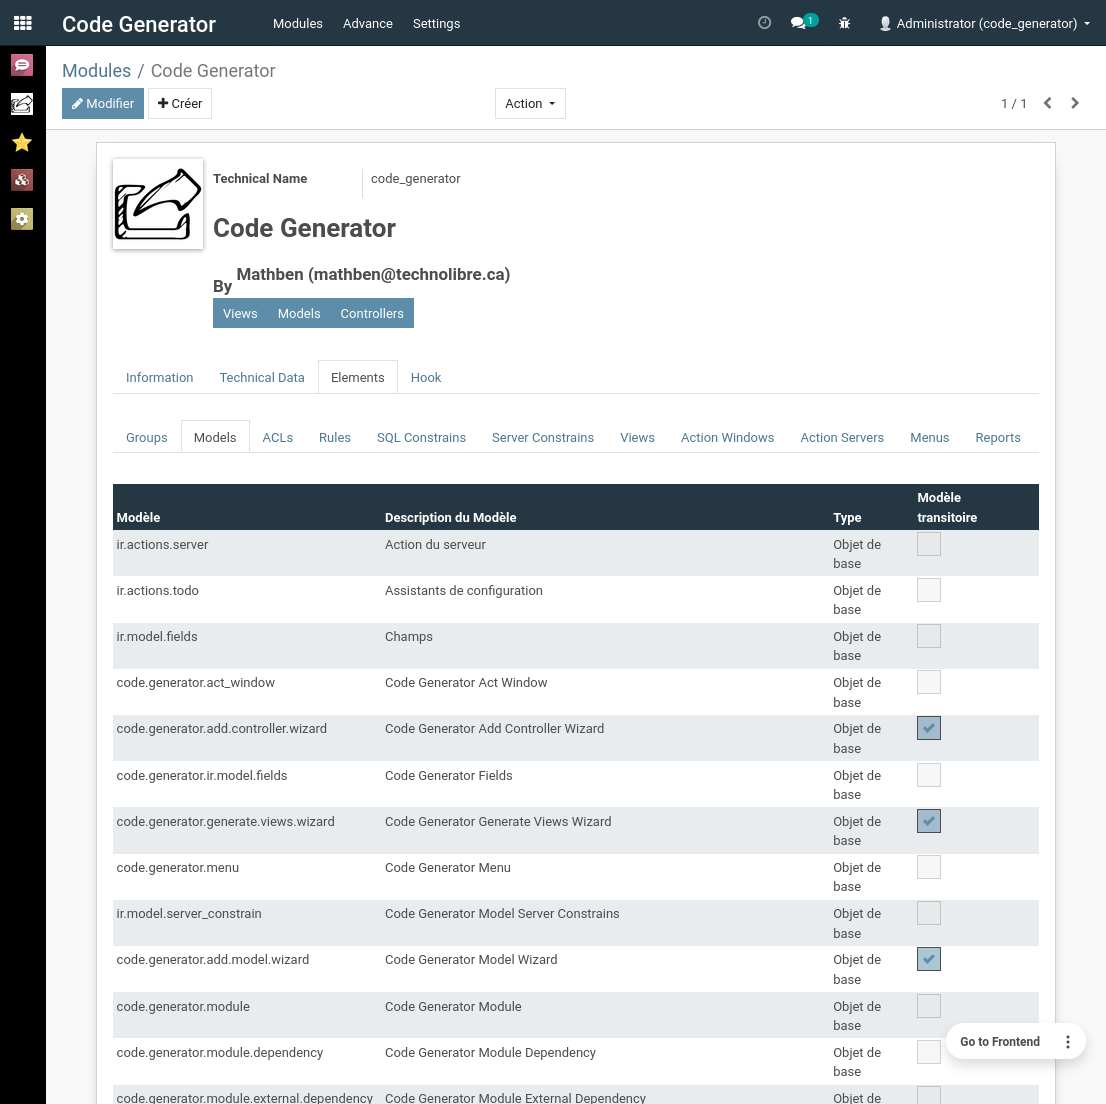
\includegraphics[width=6.535in]{cg_model.png}
\end{figure}

\Annexe{GUI générateur de code - les champs} \label{annexe_cg_gui_champs}

\begin{figure}[htb]
\centering
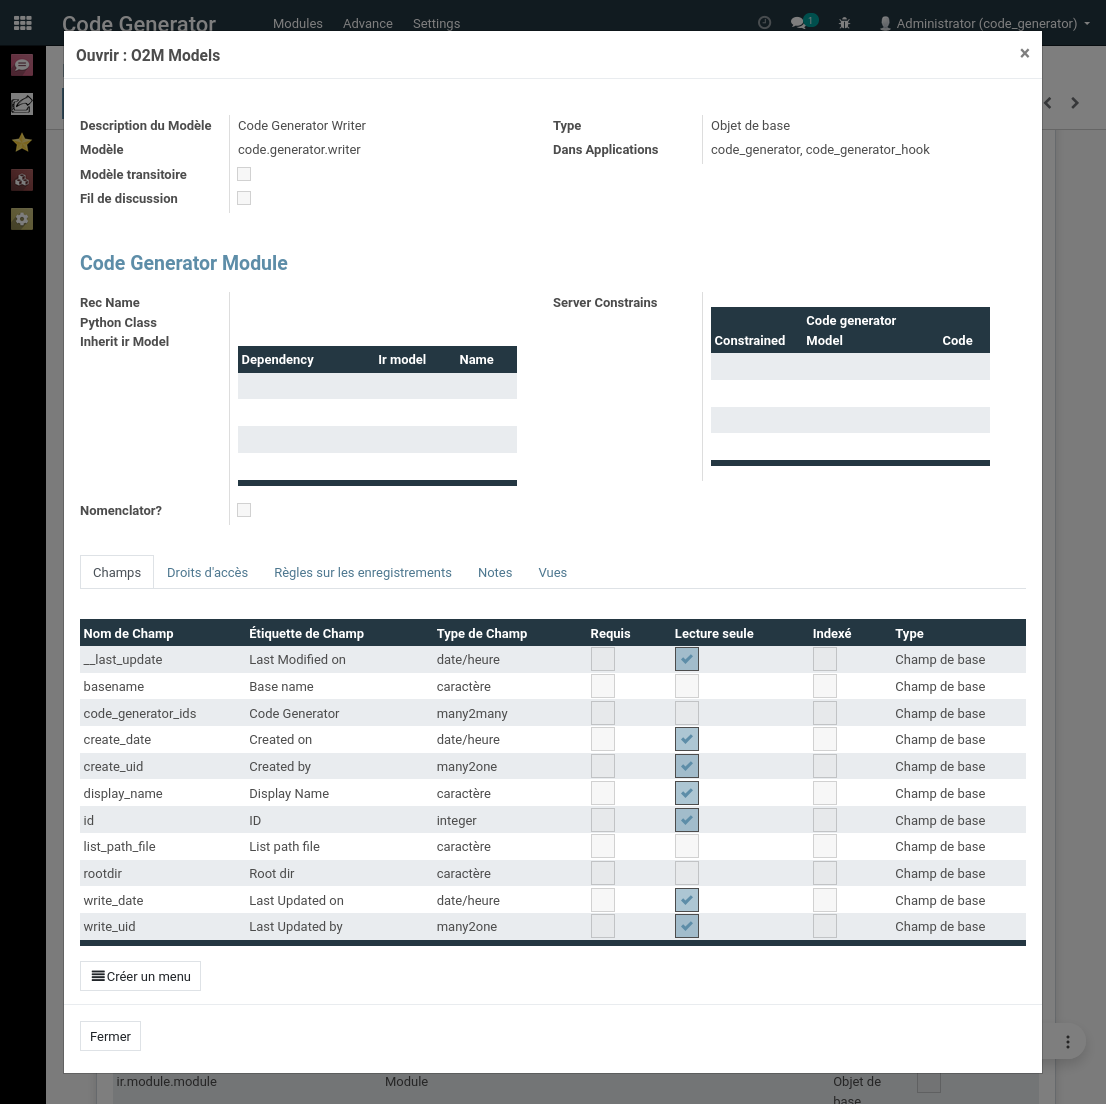
\includegraphics[width=6.535in]{cg_champs.png}
\end{figure}

\Annexe{GUI générateur de code - les codes} \label{annexe_cg_gui_code}

\begin{figure}[htb]
\centering
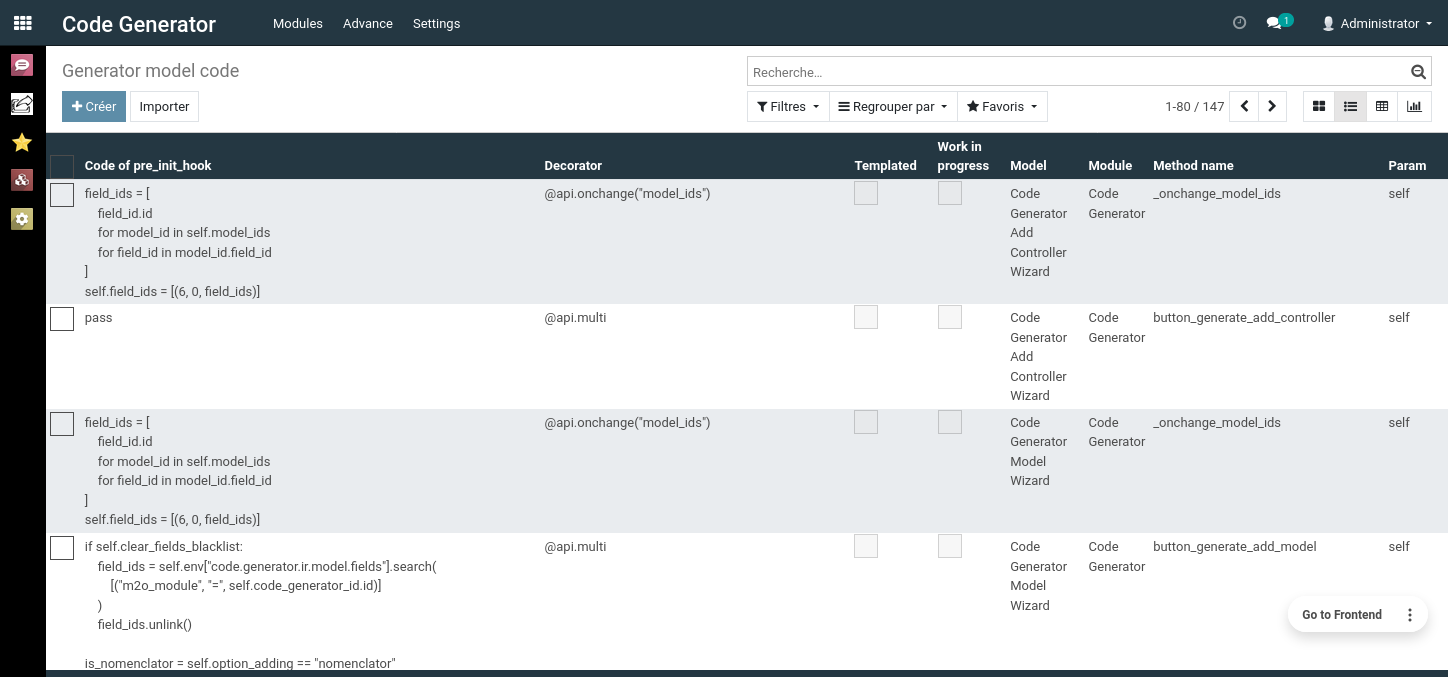
\includegraphics[width=6.535in]{cg_code.png}
\end{figure}

\Annexe{GUI générateur de code - les «hooks»} \label{annexe_cg_gui_hook}

\begin{figure}[htb]
\centering
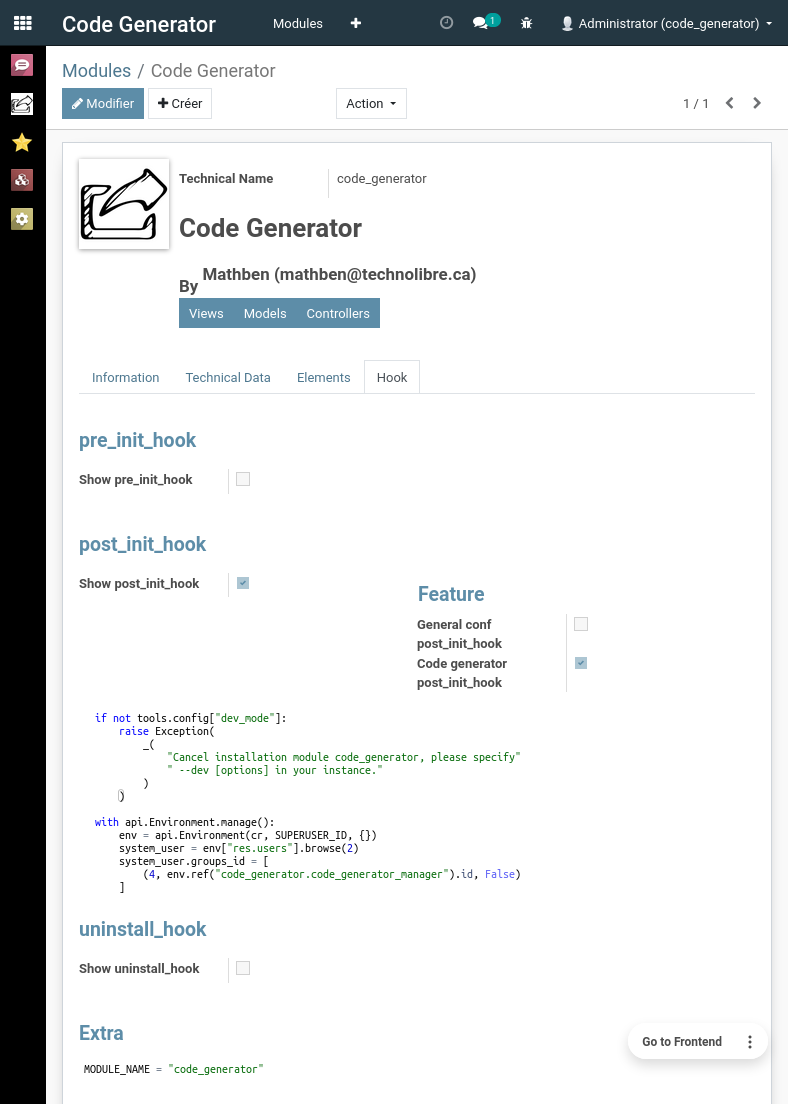
\includegraphics[height=7in]{cg_hook.png}
\end{figure}


\Annexe{Test couverture technique générateur de code} \label{annexe_test_generateur_code}

\begin{table}[htb]
\centering
\begin{tabular}{|l|l|l|l|l|l|}

\hline
\cellcolor[HTML]{d9d9d9}{\textbf{Technique}} & \multicolumn{2}{|l|}{\cellcolor[HTML]{d9d9d9}{base}} & \multicolumn{2}{|l|}{\cellcolor[HTML]{d9d9d9}{\textbf{\# instruction}}} & \cellcolor[HTML]{d9d9d9}{5 085}\\\hline

\multicolumn{2}{|l|}{\cellcolor[HTML]{efefef}{\textbf{Description du test}}} & \cellcolor[HTML]{efefef}{\textbf{Status}} & \cellcolor[HTML]{efefef}{\textbf{Durée (s)}} & \cellcolor[HTML]{efefef}{\textbf{\# de Miss}} & \cellcolor[HTML]{efefef}{\textbf{Cover (\%)}}\\\hline

\multicolumn{2}{|l|}{\shortstack[l]{Génération µ$_C^B$ modèle simple}} & Succès & 27 & 2 983 & 41\\\hline

\multicolumn{2}{|l|}{\shortstack[l]{Génération µ$_C^B$ modèle simple avec \\ héritage}} & Succès & 26 & 3 452 & 32\\\hline

\multicolumn{2}{|l|}{\shortstack[l]{Exportation µ$_C^B$ données «helpdesk»}} & Succès & 28 & 3 900 & 23\\\hline

% \end{tabular}
% \end{table}
% \begin{table}
% \centering
% \begin{tabular}{|l|l|l|l|l|l|}
% \hline

\cellcolor[HTML]{d9d9d9}{\textbf{Technique}} & \multicolumn{2}{|l|}{\cellcolor[HTML]{d9d9d9}{base + hook}} & \multicolumn{2}{|l|}{\cellcolor[HTML]{d9d9d9}{\textbf{\# instruction}}} & \cellcolor[HTML]{d9d9d9}{5 985}\\\hline

\multicolumn{2}{|l|}{\cellcolor[HTML]{efefef}{\textbf{Description du test}}} & \cellcolor[HTML]{efefef}{\textbf{Status}} & \cellcolor[HTML]{efefef}{\textbf{Durée (s)}} & \cellcolor[HTML]{efefef}{\textbf{\# de Miss}} & \cellcolor[HTML]{efefef}{\textbf{Cover (\%)}}\\\hline

\multicolumn{2}{|l|}{\shortstack[l]{Auto-génération µ$_C^0$}} & Succès & 17 & 4 683 & 22\\\hline

\multicolumn{2}{|l|}{\shortstack[l]{Nouveau projet µ$_C^0$ µ$_C^A$ µ$_C^B$ \\ «Hello World»}} & Succès & 39 & 4 610 & 23\\\hline

\multicolumn{2}{|l|}{\shortstack[l]{Génération µ$_C^A$ portail}} & Succès & 44 & 3 638 & 39\\\hline

\multicolumn{2}{|l|}{\shortstack[l]{Génération µ$_C^A$ modèle simple}} & Succès & 33 & 3 982 & 33\\\hline

\multicolumn{2}{|l|}{\shortstack[l]{Génération µ$_C^A$ modèle simple avec \\ héritage}} & Succès & 32 & 4 027 & 33\\\hline

\multicolumn{2}{|l|}{\shortstack[l]{Exportation µ$_C^B$ données «website»}} & Succès & 28 & 3 900 & 23\\\hline

\multicolumn{2}{|l|}{\shortstack[l]{Génération µ$_C^B$ du générateur de \\ code}} & Échec & 20 & 3 529 & 41\\\hline

\multicolumn{2}{|l|}{\shortstack[l]{Génération µ$_C^A$ du générateur de \\ code}} & Échec & 29 & 3 690 & 38\\\hline

% \end{tabular}
% \end{table}
% \begin{table}
% \centering
% \begin{tabular}{|l|l|l|l|l|l|}
% \hline

\cellcolor[HTML]{d9d9d9}{\textbf{Technique}} & \multicolumn{2}{|l|}{\cellcolor[HTML]{d9d9d9}{base + cron}} & \multicolumn{2}{|l|}{\cellcolor[HTML]{d9d9d9}{\textbf{\# instruction}}} & \cellcolor[HTML]{d9d9d9}{6 153}\\\hline

\multicolumn{2}{|l|}{\cellcolor[HTML]{efefef}{\textbf{Description du test}}} & \cellcolor[HTML]{efefef}{\textbf{Status}} & \cellcolor[HTML]{efefef}{\textbf{Durée (s)}} & \cellcolor[HTML]{efefef}{\textbf{\# de Miss}} & \cellcolor[HTML]{efefef}{\textbf{Cover (\%)}}\\\hline

\multicolumn{2}{|l|}{\shortstack[l]{Génération µ$_C^A$ «auto\_backup»}} & Succès & 36 & 3 422 & 44\\\hline

% \end{tabular}
% \end{table}
% \begin{table}
% \centering
% \begin{tabular}{|l|l|l|l|l|l|}
% \hline

\cellcolor[HTML]{d9d9d9}{\textbf{Technique}} & \multicolumn{2}{|l|}{\cellcolor[HTML]{d9d9d9}{base + portal}} & \multicolumn{2}{|l|}{\cellcolor[HTML]{d9d9d9}{\textbf{\# instruction}}} & \cellcolor[HTML]{d9d9d9}{5 799}\\\hline

\multicolumn{2}{|l|}{\cellcolor[HTML]{efefef}{\textbf{Description du test}}} & \cellcolor[HTML]{efefef}{\textbf{Status}} & \cellcolor[HTML]{efefef}{\textbf{Durée (s)}} & \cellcolor[HTML]{efefef}{\textbf{\# de Miss}} & \cellcolor[HTML]{efefef}{\textbf{Cover (\%)}}\\\hline

\multicolumn{2}{|l|}{\shortstack[l]{Génération µ$_C^B$ exemple MariaDB \\ \texttt{SQL}}} & Succès & 80 & 3 104 & 46\\\hline

% \end{tabular}
% \end{table}
% \begin{table}
% \centering
% \begin{tabular}{|l|l|l|l|l|l|}
% \hline

\cellcolor[HTML]{d9d9d9}{\textbf{Technique}} & \multicolumn{2}{|l|}{\cellcolor[HTML]{d9d9d9}{base + «theme\_website»}} & \multicolumn{2}{|l|}{\cellcolor[HTML]{d9d9d9}{\textbf{\# instruction}}} & \cellcolor[HTML]{d9d9d9}{5 336}\\\hline

\multicolumn{2}{|l|}{\cellcolor[HTML]{efefef}{\textbf{Description du test}}} & \cellcolor[HTML]{efefef}{\textbf{Status}} & \cellcolor[HTML]{efefef}{\textbf{Durée (s)}} & \cellcolor[HTML]{efefef}{\textbf{\# de Miss}} & \cellcolor[HTML]{efefef}{\textbf{Cover (\%)}}\\\hline

\multicolumn{2}{|l|}{\shortstack[l]{Génération µ$_C^B$ thème «website»}} & Succès & 27 & 3 938 & 26\\\hline

% \end{tabular}
% \end{table}
% \begin{table}
% \centering
% \begin{tabular}{|l|l|l|l|l|l|}
% \hline

\cellcolor[HTML]{d9d9d9}{\textbf{Technique}} & \multicolumn{2}{|l|}{\cellcolor[HTML]{d9d9d9}{base + «website\_snippet»}} & \multicolumn{2}{|l|}{\cellcolor[HTML]{d9d9d9}{\textbf{\# instruction}}} & \cellcolor[HTML]{d9d9d9}{5 615}\\\hline

\multicolumn{2}{|l|}{\cellcolor[HTML]{efefef}{\textbf{Description du test}}} & \cellcolor[HTML]{efefef}{\textbf{Status}} & \cellcolor[HTML]{efefef}{\textbf{Durée (s)}} & \cellcolor[HTML]{efefef}{\textbf{\# de Miss}} & \cellcolor[HTML]{efefef}{\textbf{Cover (\%)}}\\\hline

\multicolumn{2}{|l|}{\shortstack[l]{Génération µ$_C^B$ individuel \\ «website\_snippet»}} & Succès & 26 & 4 284 & 24\\\hline

\end{tabular}
\end{table}
\begin{table}[htb]
\centering
\begin{tabular}{|l|l|l|l|l|l|}
\hline

\cellcolor[HTML]{d9d9d9}{\textbf{Technique}} & \multicolumn{2}{|l|}{\cellcolor[HTML]{d9d9d9}{\shortstack[l]{base + portal + \\ «website\_snippet»}}} & \multicolumn{2}{|l|}{\cellcolor[HTML]{d9d9d9}{\textbf{\# instruction}}} & \cellcolor[HTML]{d9d9d9}{6 329}\\\hline

\multicolumn{2}{|l|}{\cellcolor[HTML]{efefef}{\textbf{Description du test}}} & \cellcolor[HTML]{efefef}{\textbf{Status}} & \cellcolor[HTML]{efefef}{\textbf{Durée (s)}} & \cellcolor[HTML]{efefef}{\textbf{\# de Miss}} & \cellcolor[HTML]{efefef}{\textbf{Cover (\%)}}\\\hline

\multicolumn{2}{|l|}{\shortstack[l]{Génération µ$_C^B$ multiple \\ «website\_snippet»}} & Succès & 36 & 2 898 & 54\\\hline

\multicolumn{2}{|l|}{\shortstack[l]{Génération µ$_C^B$ portail}} & Succès & 34 & 3 173 & 50\\\hline

% \end{tabular}
% \end{table}
% \begin{table}
% \centering
% \begin{tabular}{|l|l|l|l|l|l|}
% \hline

\cellcolor[HTML]{d9d9d9}{\textbf{Technique}} & \multicolumn{2}{|l|}{\cellcolor[HTML]{d9d9d9}{base + portal + «Migration DB»}} & \multicolumn{2}{|l|}{\cellcolor[HTML]{d9d9d9}{\textbf{\# instruction}}} & \cellcolor[HTML]{d9d9d9}{6 559}\\\hline

\multicolumn{2}{|l|}{\cellcolor[HTML]{efefef}{\textbf{Description du test}}} & \cellcolor[HTML]{efefef}{\textbf{Status}} & \cellcolor[HTML]{efefef}{\textbf{Durée (s)}} & \cellcolor[HTML]{efefef}{\textbf{\# de Miss}} & \cellcolor[HTML]{efefef}{\textbf{Cover (\%)}}\\\hline

\multicolumn{2}{|l|}{\shortstack[l]{Génération migration MariaDB \\ \texttt{SQL}}} & Succès & 121 & 3 267 & 50\\\hline

% \end{tabular}
% \end{table}
% \begin{table}
% \centering
% \begin{tabular}{|l|l|l|l|l|l|}

\hline
\cellcolor[HTML]{d9d9d9}{\textbf{Technique}} & \multicolumn{2}{|l|}{\cellcolor[HTML]{d9d9d9}{base + hook + portal}} & \multicolumn{2}{|l|}{\cellcolor[HTML]{d9d9d9}{\textbf{\# instruction}}} & \cellcolor[HTML]{d9d9d9}{6 699}\\\hline

\multicolumn{2}{|l|}{\cellcolor[HTML]{efefef}{\textbf{Description du test}}} & \cellcolor[HTML]{efefef}{\textbf{Status}} & \cellcolor[HTML]{efefef}{\textbf{Durée (s)}} & \cellcolor[HTML]{efefef}{\textbf{\# de Miss}} & \cellcolor[HTML]{efefef}{\textbf{Cover (\%)}}\\\hline

\multicolumn{2}{|l|}{\shortstack[l]{Génération µ$_C^A$ MariaDB \texttt{SQL}}} & Succès & 78 & 4 315 & 36\\\hline

% \end{tabular}
% \end{table}
% \begin{table}
% \centering
% \begin{tabular}{|l|l|l|l|l|l|}
% \hline

\cellcolor[HTML]{d9d9d9}{\textbf{Technique}} & \multicolumn{2}{|l|}{\cellcolor[HTML]{d9d9d9}{base + hook + cron}} & \multicolumn{2}{|l|}{\cellcolor[HTML]{d9d9d9}{\textbf{\# instruction}}} & \cellcolor[HTML]{d9d9d9}{6 153}\\\hline

\multicolumn{2}{|l|}{\cellcolor[HTML]{efefef}{\textbf{Description du test}}} & \cellcolor[HTML]{efefef}{\textbf{Status}} & \cellcolor[HTML]{efefef}{\textbf{Durée (s)}} & \cellcolor[HTML]{efefef}{\textbf{\# de Miss}} & \cellcolor[HTML]{efefef}{\textbf{Cover (\%)}}\\\hline

\multicolumn{2}{|l|}{\shortstack[l]{Génération µ$_C^A$ «auto\_backup»}} & Succès & 36 & 3 422 & 44\\\hline

% \end{tabular}
% \end{table}
% \begin{table}
% \centering
% \begin{tabular}{|l|l|l|l|l|l|}
% \hline

\cellcolor[HTML]{d9d9d9}{\textbf{Technique}} & \multicolumn{2}{|l|}{\cellcolor[HTML]{d9d9d9}{\shortstack[l]{base + geoengine + \\ «website\_leaflet»}}} & \multicolumn{2}{|l|}{\cellcolor[HTML]{d9d9d9}{\textbf{\# instruction}}} & \cellcolor[HTML]{d9d9d9}{5 423}\\\hline

\multicolumn{2}{|l|}{\cellcolor[HTML]{efefef}{\textbf{Description du test}}} & \cellcolor[HTML]{efefef}{\textbf{Status}} & \cellcolor[HTML]{efefef}{\textbf{Durée (s)}} & \cellcolor[HTML]{efefef}{\textbf{\# de Miss}} & \cellcolor[HTML]{efefef}{\textbf{Cover (\%)}}\\\hline

\multicolumn{2}{|l|}{\shortstack[l]{Génération µ$_C^B$ \\ «website\_snippet\_leaflet»}} & Succès & 33 & 3 259 & 40\\\hline

% \end{tabular}
% \end{table}
% \begin{table}
% \centering
% \begin{tabular}{|l|l|l|l|l|l|}
% \hline

\cellcolor[HTML]{d9d9d9}{\textbf{Technique}} & \multicolumn{2}{|l|}{\cellcolor[HTML]{d9d9d9}{\shortstack[l]{base + cron + hook + \\ «Migration DB» + geoengine + \\ portal + «theme\_website» + \\ «website\_snippet» + \\ «website\_leaflet»}}} & \multicolumn{2}{|l|}{\cellcolor[HTML]{d9d9d9}{\textbf{\# instruction}}} & \cellcolor[HTML]{d9d9d9}{8 746}\\\hline

\multicolumn{2}{|l|}{\cellcolor[HTML]{efefef}{\textbf{Description du test}}} & \cellcolor[HTML]{efefef}{\textbf{Status}} & \cellcolor[HTML]{efefef}{\textbf{Durée (s)}} & \cellcolor[HTML]{efefef}{\textbf{\# de Miss}} & \cellcolor[HTML]{efefef}{\textbf{Cover (\%)}}\\\hline

\multicolumn{2}{|l|}{\shortstack[l]{Tous les tests à succès}} & Succès & 194 & 1 371 & 84\\\hline

\end{tabular}
\end{table}

\Annexe{Diagramme modèle de données Espace Membre Accorderie 2019} \label{annexe_db_accorderie_2019}

\begin{figure}[htb]
\centering
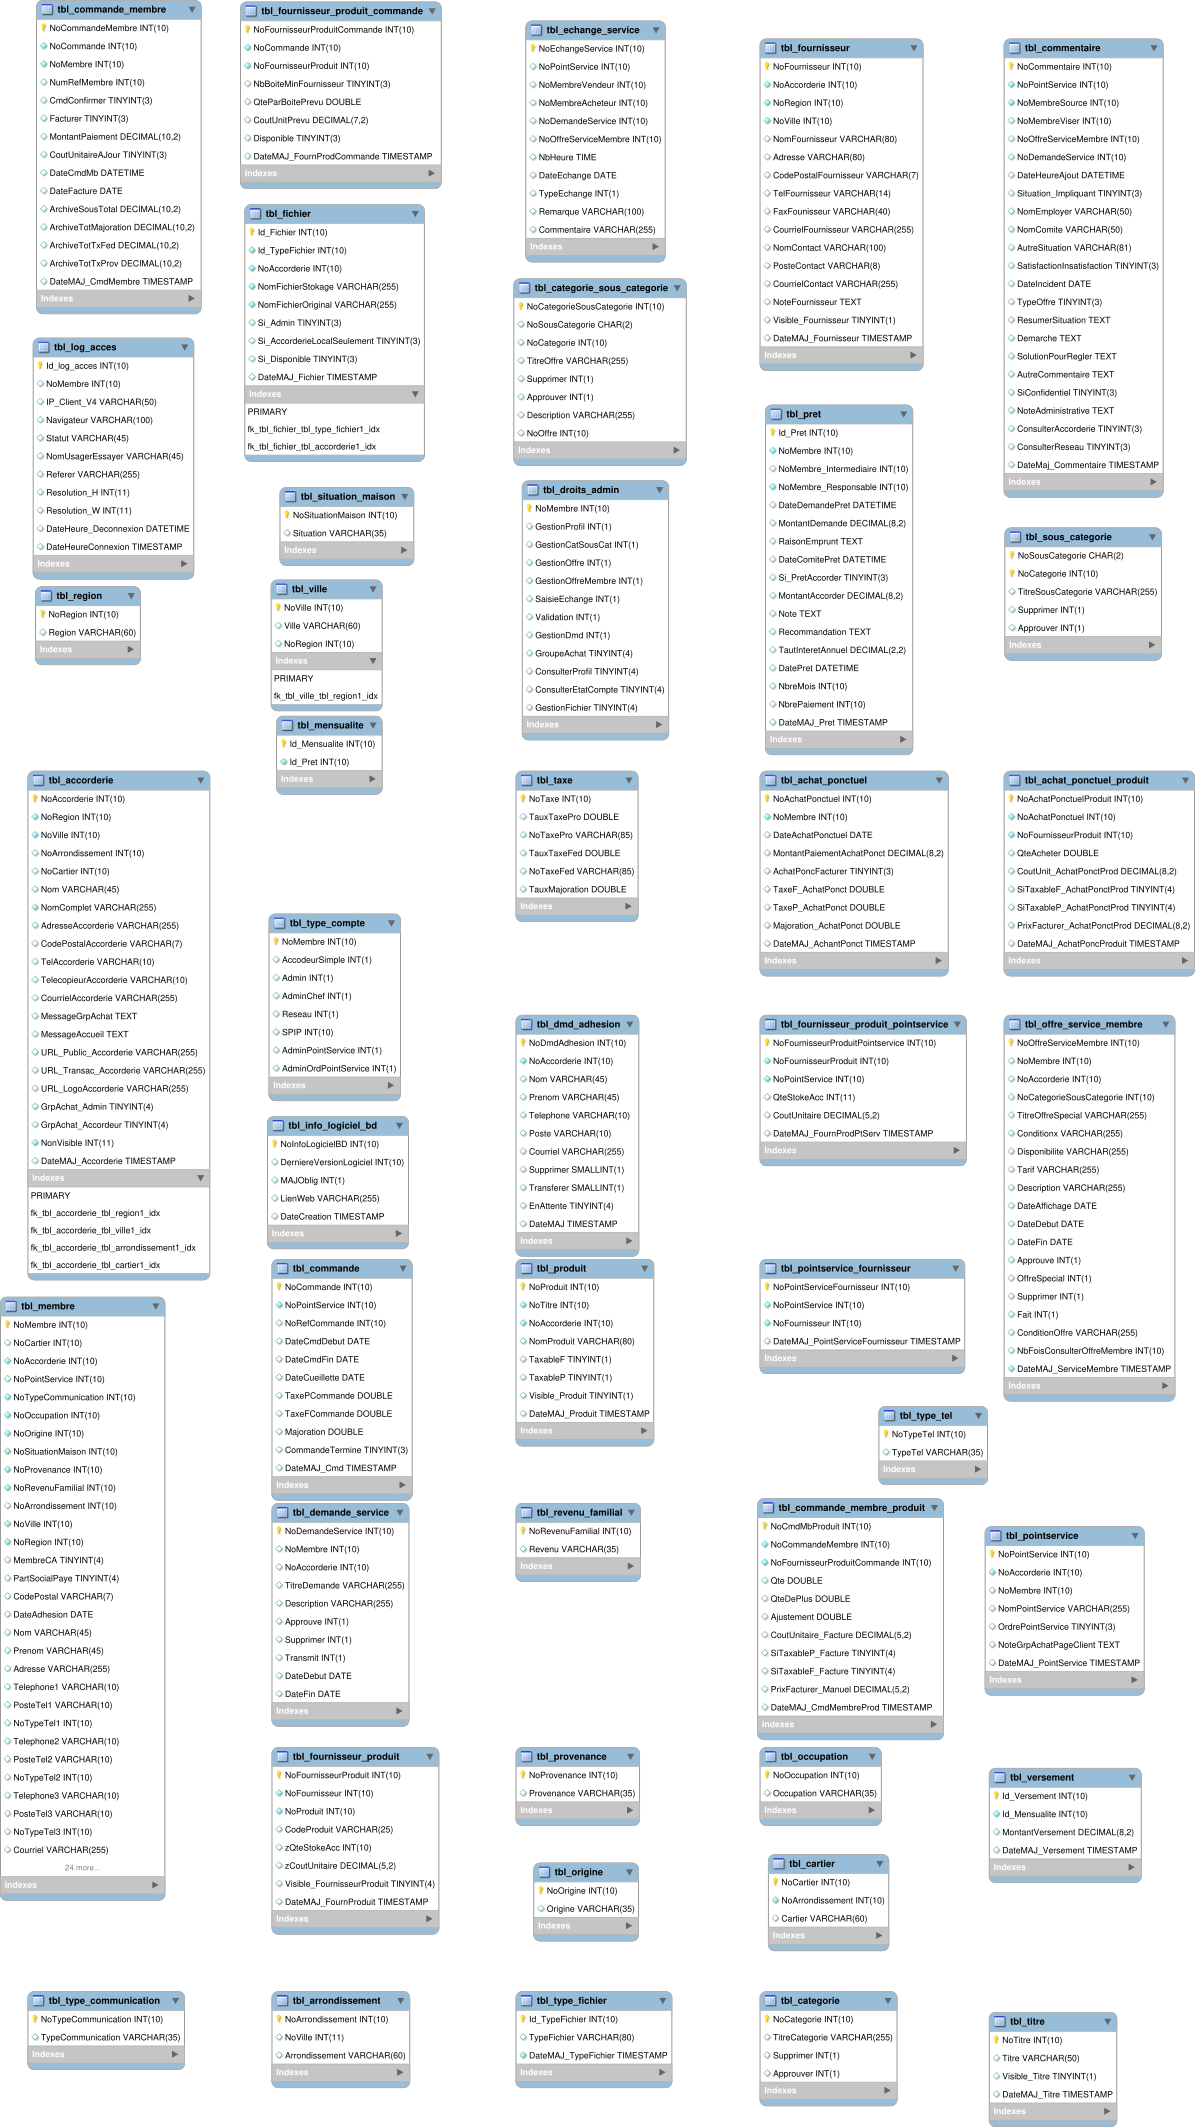
\includegraphics[height=7in]{schema_bd_accorderie.png}
\end{figure}

\Annexe{Diagramme nouveau modèle de données Espace Membre Accorderie 2023} \label{annexe_db_accorderie_2023}

\begin{figure}[htb]
\centering
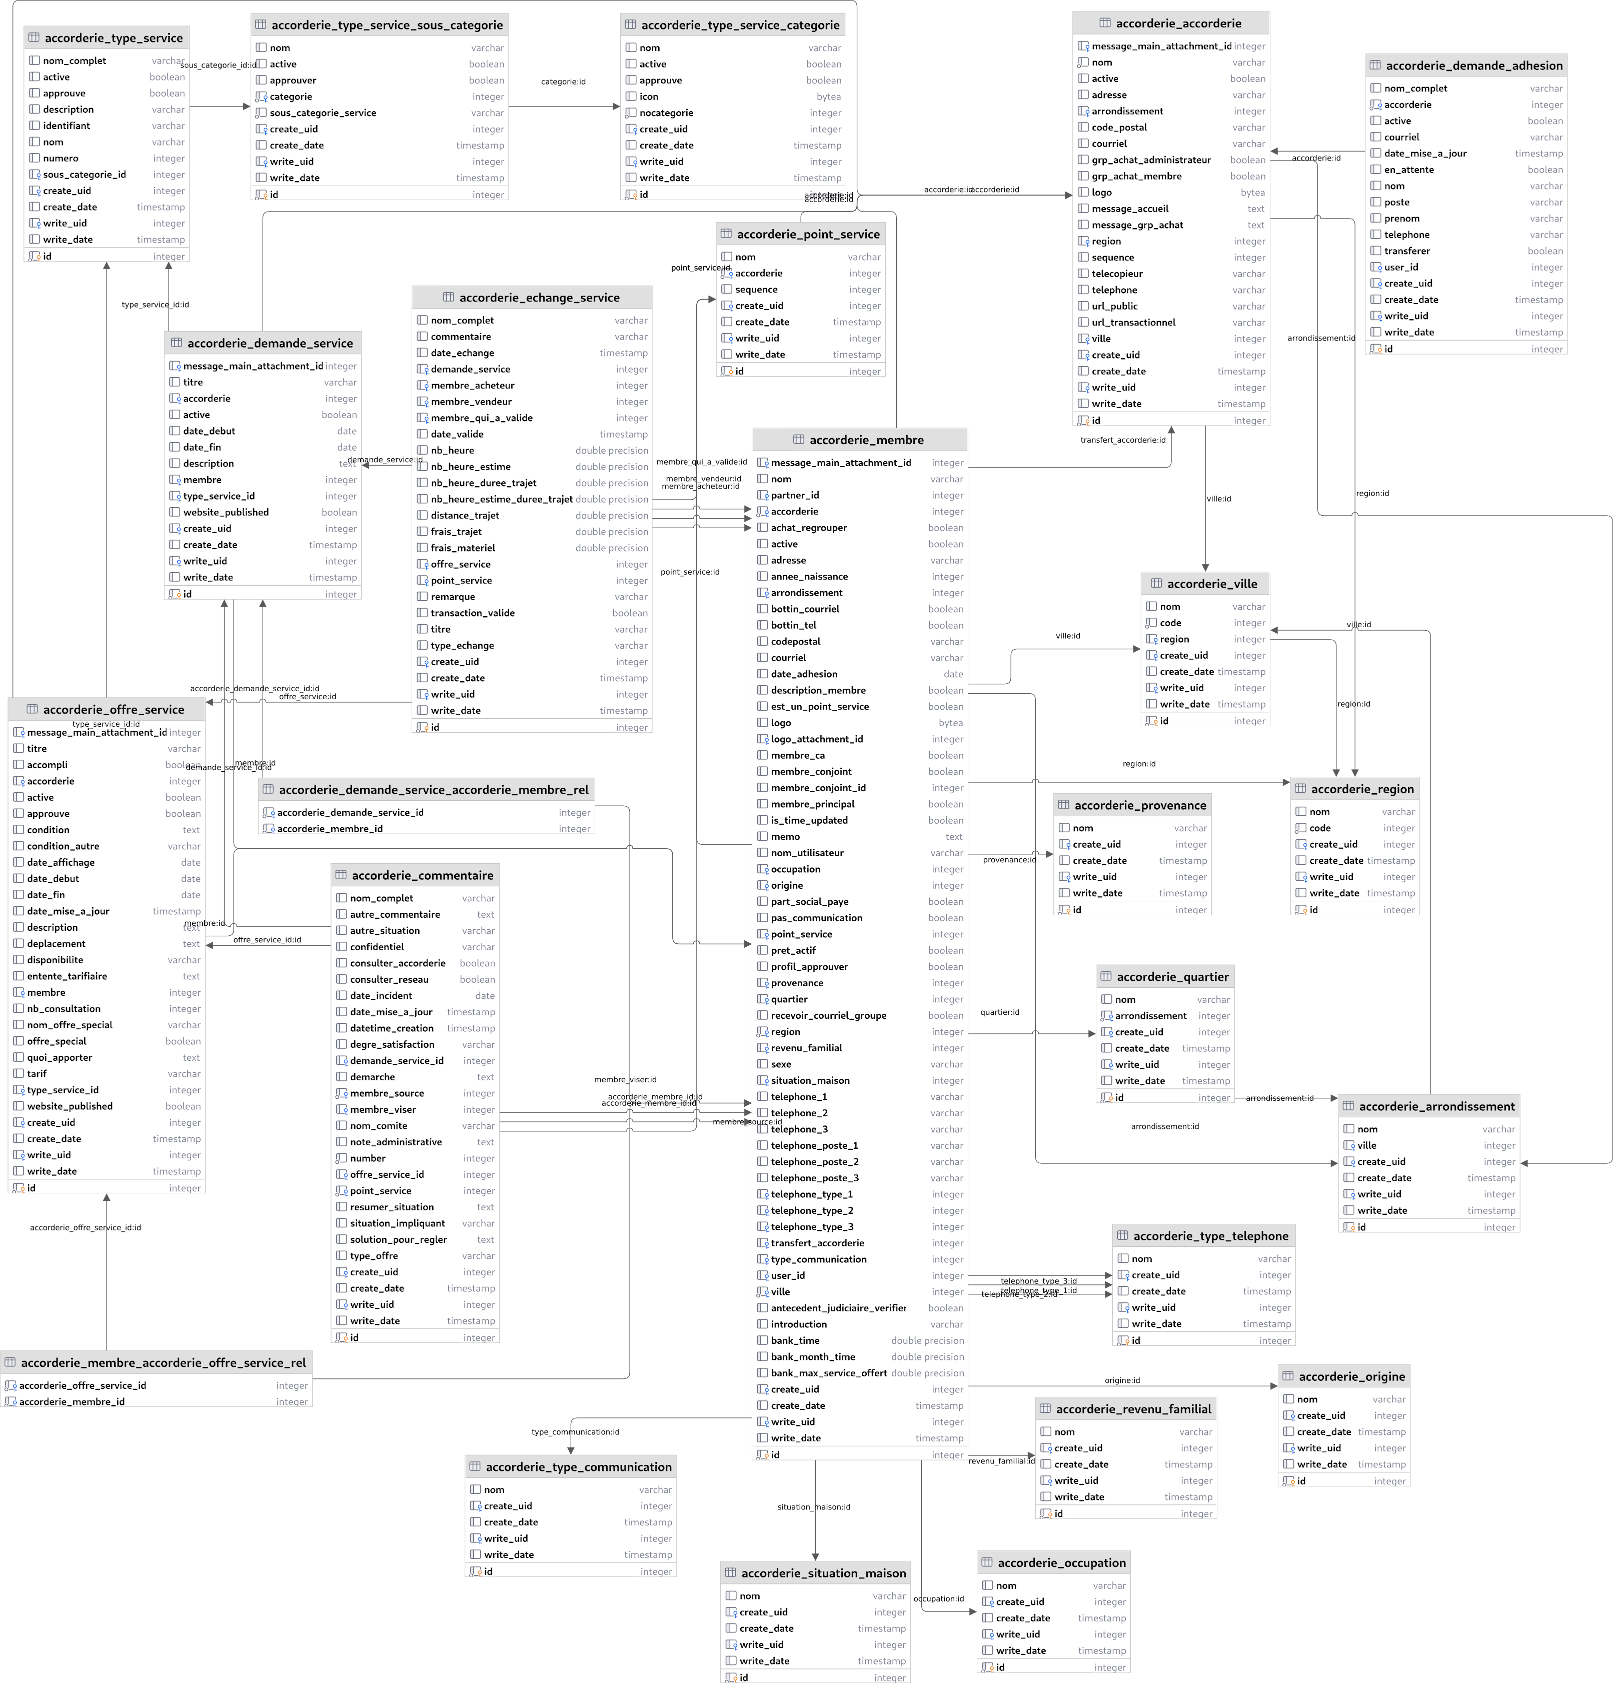
\includegraphics[width=6.535in]{schema_bd_accorderie_new_small.png}
\end{figure}

\Annexe{Diagramme processus pour demander, offrir, établir un échange et le valider - Accorderie 2023} \label{annexe_processus_accorderie_2023}

\begin{figure}[htb]
\centering
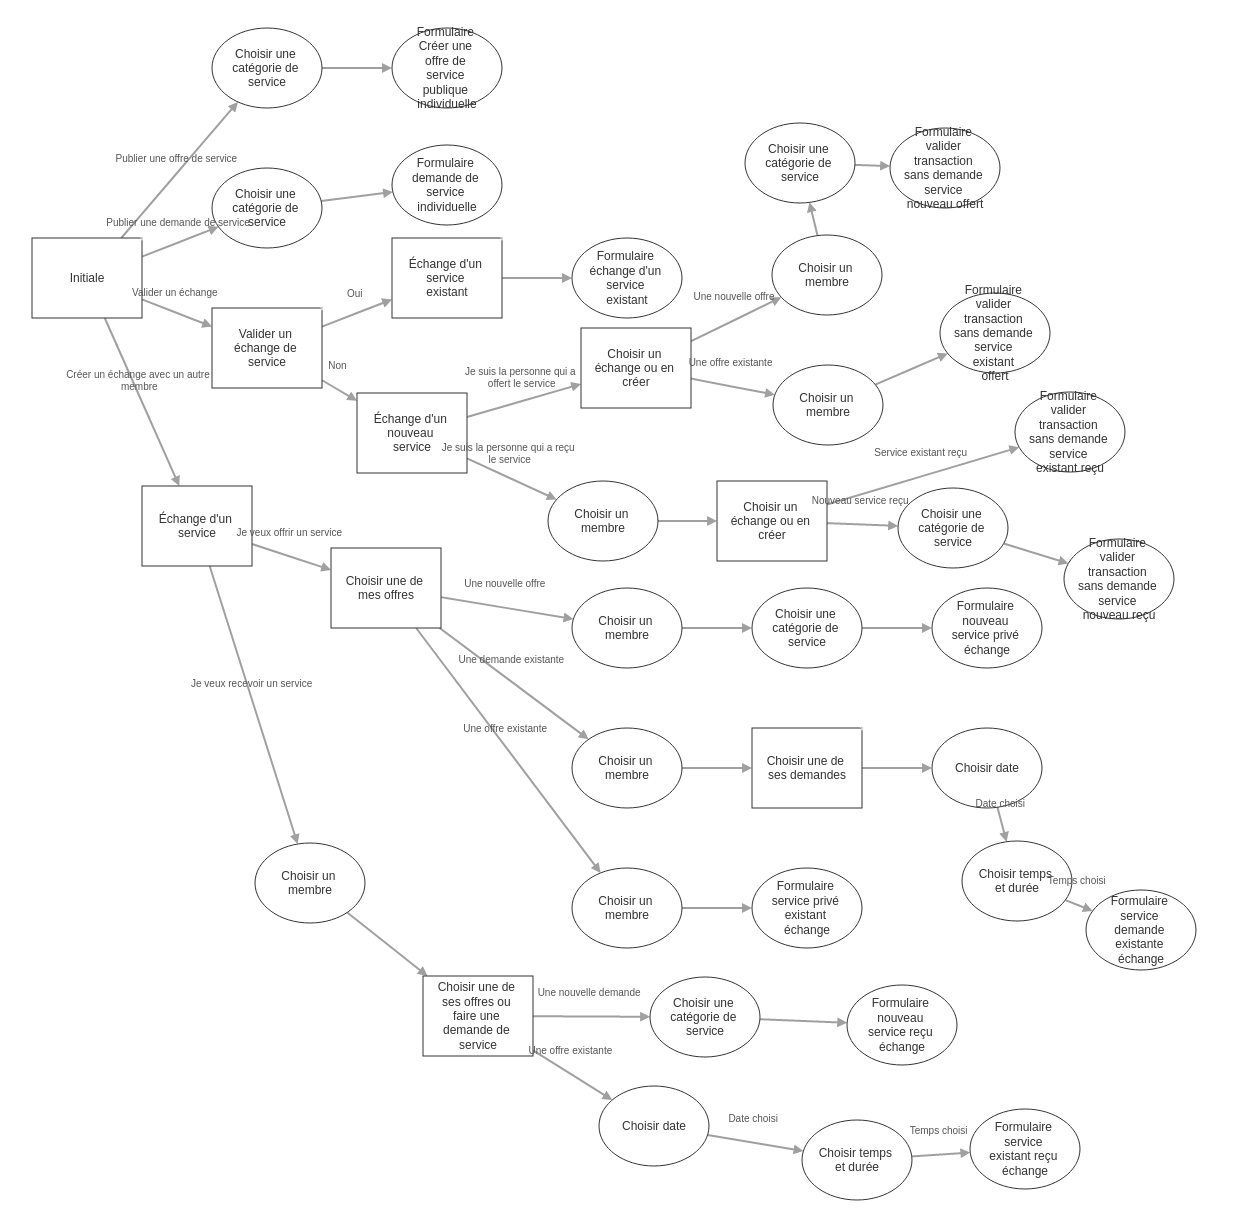
\includegraphics[width=6.535in]{accorderie_processus.png}
\end{figure}

\Annexe{Diagramme modèle de données du portail CEPPP septembre 2022} \label{annexe_db_ceppp_2022}

\begin{figure}[htb]
\centering
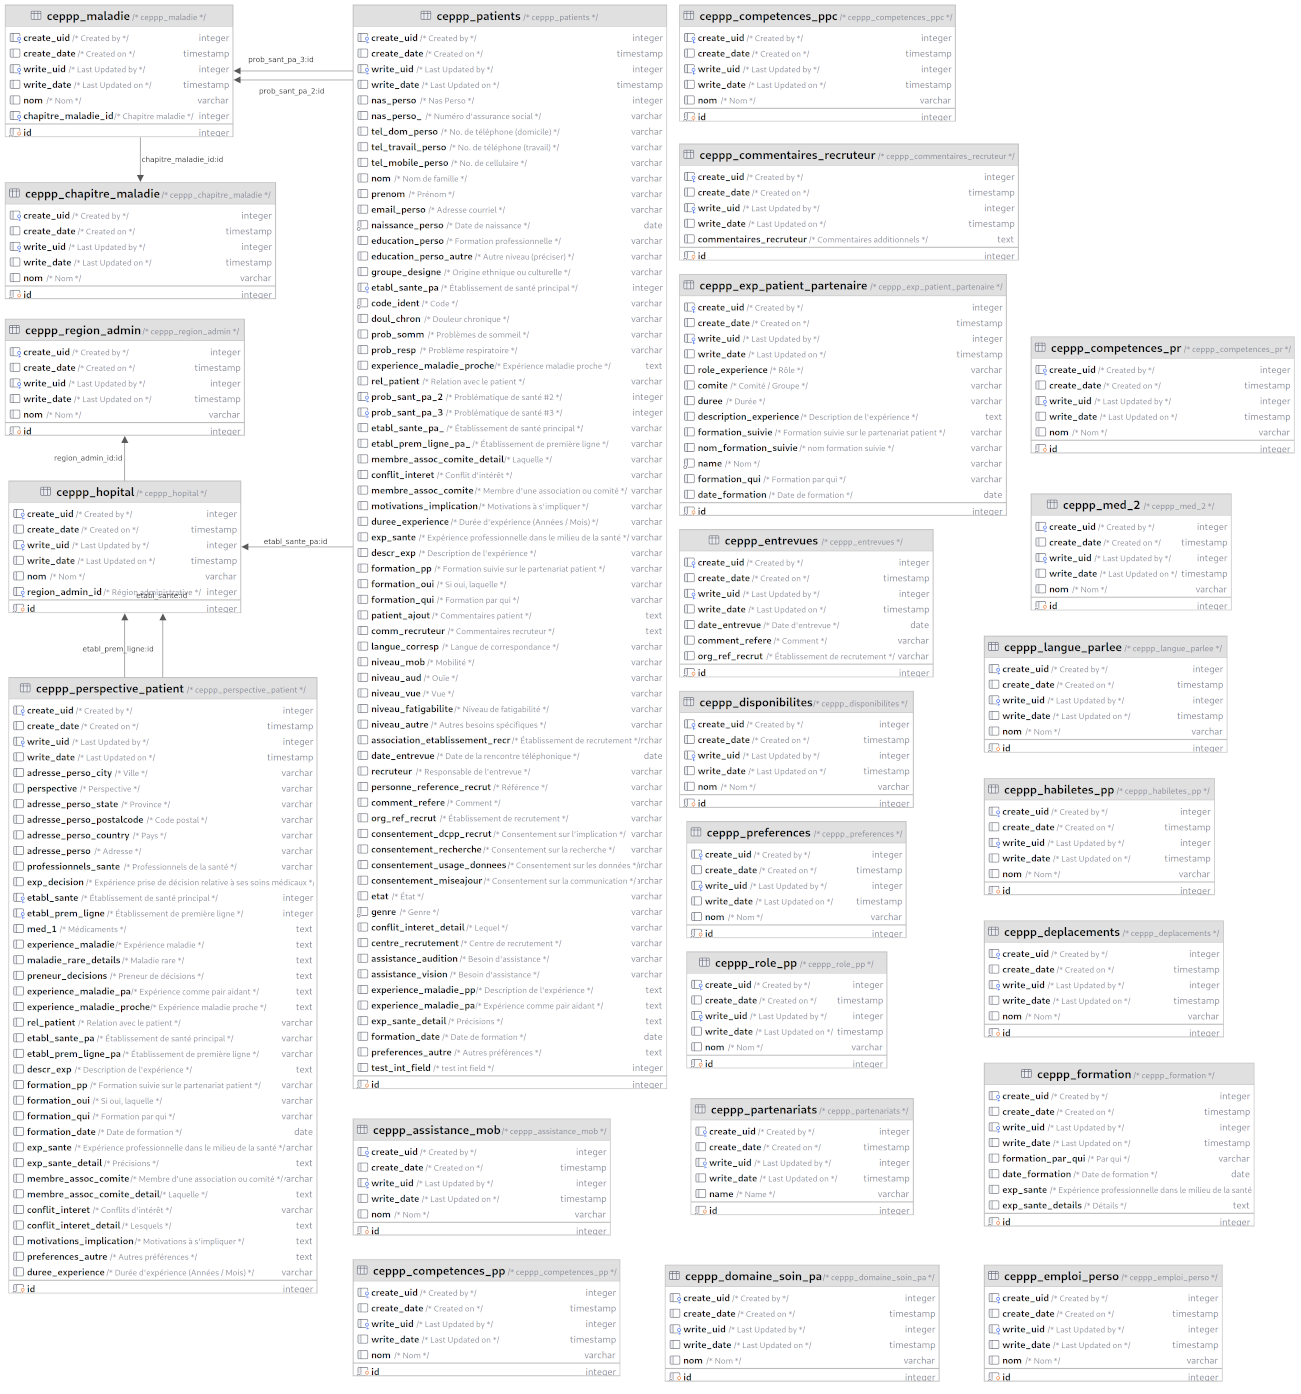
\includegraphics[width=6.535in]{schema_bd_ceppp_suite_crm_small.png}
\end{figure}

\Annexe{Vue formulaire administration portail CEPPP} \label{annexe_form_ceppp_2022}

\begin{figure}[htb]
\centering
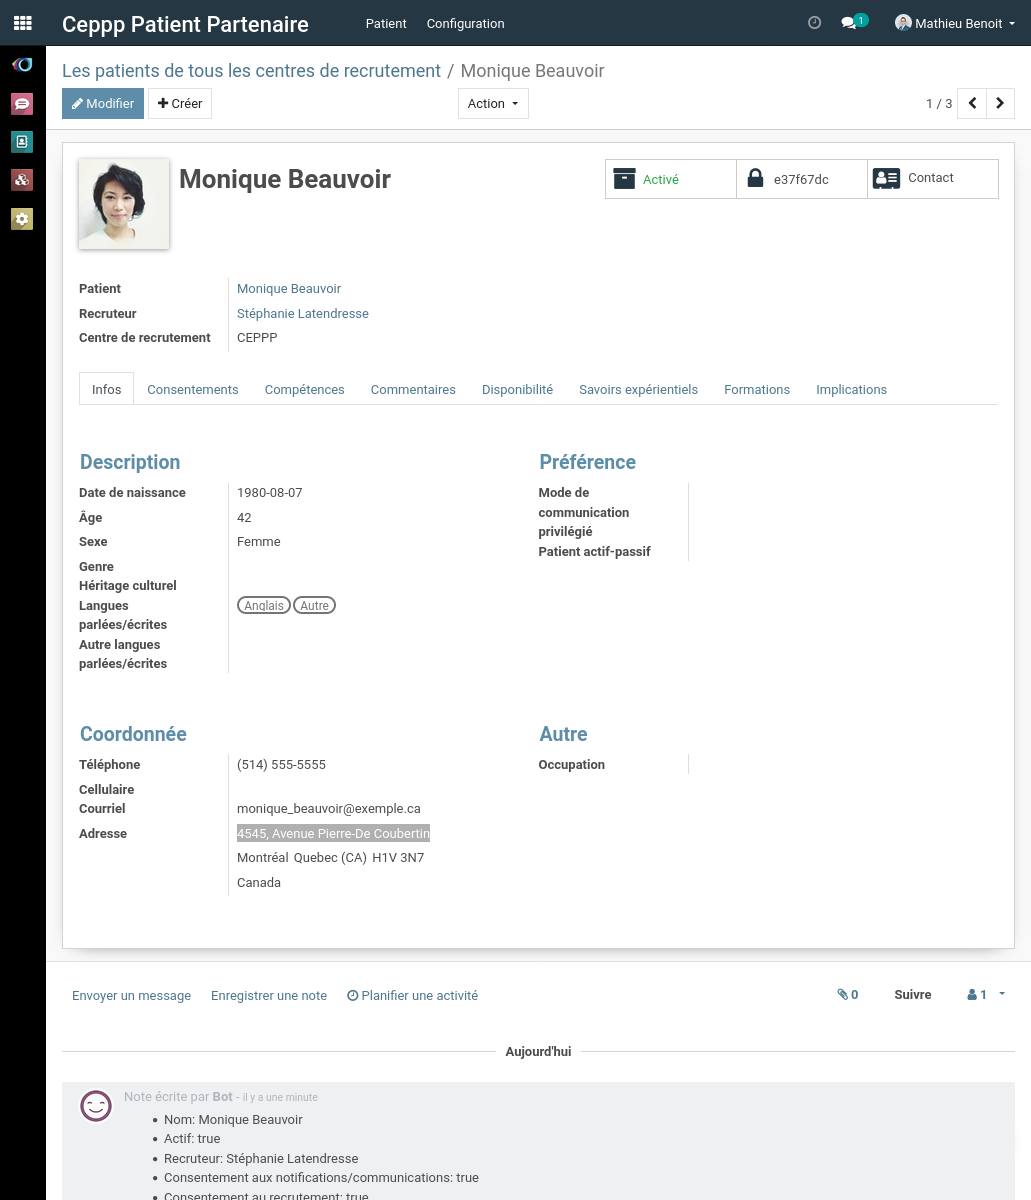
\includegraphics[height=7in]{exemple_vue_formulaire_patient_ceppp.png}
\end{figure}

\Annexe{Vue formulaire partenaire portail CEPPP} \label{annexe_form_anonyme_ceppp_2022}

\begin{figure}[htb]
\centering
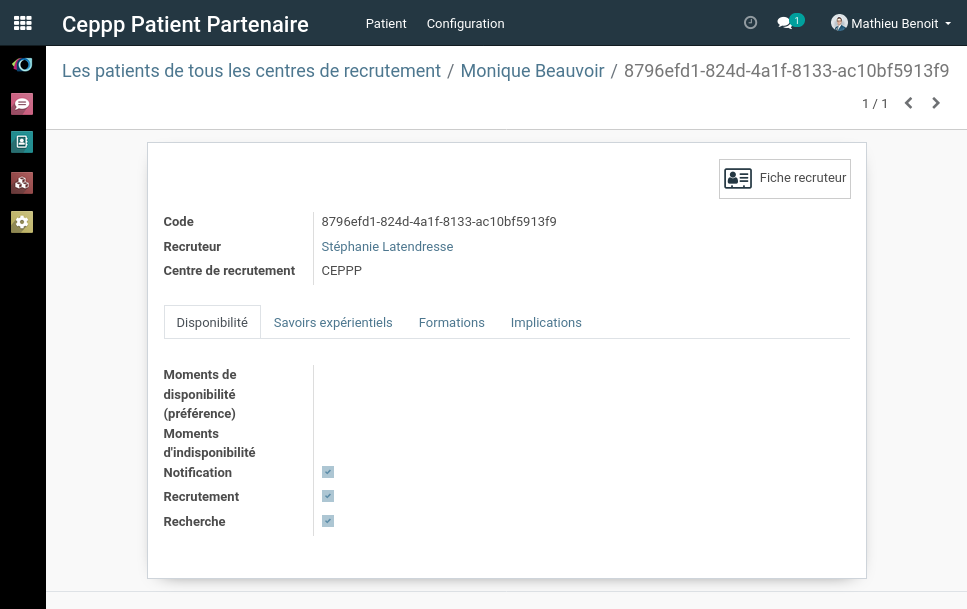
\includegraphics[width=6.535in]{exemple_vue_formulaire_patient_anonyme_ceppp.png}
\end{figure}
}
{}
\end{document}
